%!TEX options = --shell-escape


\documentclass[bachelor]{thesis-uestc}
%----文内引用符号
\usepackage[utf8]{inputenc}
\usepackage{cleveref}
\crefname{section}{§}{§§}
%----------

\title{密文重复数据删除机制的频率攻击方法}
\author{任彦璟}
\advisor{李经纬\chinesespace 副教授}
\school{计算机科学与工程学院(网络空间安全学院)}
\major{信息安全}
\studentid{2015040101018}

\begin{document}

\makecover

\begin{chineseabstract}

加密重复数据删除旨在解决大规模数据存储系统中的安全性和存储效率:它确保每个明文都由明文本身内容派生的对称密钥加密,从而为数据存储提供机密性保证,同时保留重复数据删除的存储节省效率。但是,加密重复数据删除的确定性特性也会泄漏明文的频率,从而使加密重复数据删除容易受到频率分析的影响。在本文中,我们重新审视了频率分析导致的加密重复数据删除的安全漏洞。我们认为加密重复数据删除可能更容易受到精心设计的频率分析攻击,因此攻击提供了高可信度,可确保每个推断的明文确实对应于目标密文的概率很高(即从统计角度来看,高精度) 。为此,我们提出了两种新的频率分析攻击,它们可以适应实际重复数据删除工作负载的特性,从而提高频率分析的准确性。我们根据实际情况评估针对实际存储工作负载的建议攻击,并提供有关如何带来实际损失的观察。

\chinesekeyword{加密重复数据删除, 频率分析攻击, 聚类分析}
\end{chineseabstract}

\begin{englishabstract}
Encrypted deduplication aims to address security and storage efficiency in large-scale data storage systems: it ensures that each plaintext is encrypted by a symmetric key that is derived from the content of the plaintext itself, so as to provide confidentiality guarantees for data storage while preserving the storage saving effectiveness of deduplication. However, the deterministic nature of encrypted deduplication also leaks the frequencies of plaintexts, thereby making encrypted deduplication vulnerable to frequency analysis. In this paper, we revisit the security vulnerability of encrypted deduplication due to frequency analysis. We argue that encrypted deduplication can be even more vulnerable to carefully crafted frequency analysis attacks, such that the attacks provide high confidence of ensuring that each inferred plaintext indeed corresponds to the target ciphertext with a high probability (i.e., high precision from a statistical perspective). To this end, we propose two new frequency analysis attacks that adapt the characteristics of practical deduplication workloads to increasing the severity of frequency analysis. We empirically evaluate our proposed attacks against real-world storage workloads, and provide observations on how they bring actual damages.

\englishkeyword{Encrypted deduplication, Frequency analysis attacks, Cluster analysis}
\end{englishabstract}

\thesistableofcontents

\thesischapterexordium


\chapter{绪\hspace{6pt}论}

\section{研究工作的背景与意义}
\subsection{研究背景}

随着信息技术产业的高速发展,数字信息量呈爆炸式增长。Gartner研究表明\citing{gartner2015} ,仅2015年的移动数据流量就较2014年增长59\%;并且,这一增长率将持至2018年末,移动数据流量水平达1.73亿TB。数据的快速增长导致企业面临的存储和管理成本越来越高\citing{敖莉2010重复数据删除技术}。另一方面,在存储系统所保存的数据中,高达60\%的数据都是冗余的,随着时间的推移,这些冗余数据的比例将进一步上升\citing{mcknight2006digital}。近年来,存储系统中数据高冗余的特点得到越来越多研究人员的关注,利用该特点来节省存储容量是一个热门研究课题。

数据重删技术(data deduplication)是指通过识别数据流中的冗余,只传输或存储唯一数据(unique data),而使用指向已存储数据的指针替换重复副本, 以达到节省带宽或存储空间的目的\citing{2012重复数据删除关键技术研究进展}。由于能够有效地降低存储开销,数据重删技术非常适合为管理日益增长的海量数据节省成本。在工业界,EMC Data Domain\citing{EMCDataDomain}和Avamar\citing{Avamar}、Veritas的NetBackup Appliances\citing{veritas} 以及Commvault的开放数据平台\citing{CommVault} 都是比较知名的数据重删应用产品;此外,各大云存储厂商(例如 Dropbox、Google Drive、Bitcasa、Moza等)也纷纷将数据重删技术应用于各自的云服务产品中,以提升经济效益\citing{harnik2010side}。

如图\ref{fig:数据重删系统的存储模式}所示,在支持数据重删的存储系统(统称为数据重删系统)中,重删后的任何数据块都被一个或多个文件引用,而文件则以指向这些数据块的指针的集合形式存储。这种文件共用数据块的存储模式强调了数据块的敏感性,因为一个数据块的泄漏可能扩散影响到共用这个数据块的所有文件。如何保护重删后的数据的隐私,成为信息安全领域的一个研究热点。

\begin{figure}[!htb]
    \small
    \centering
    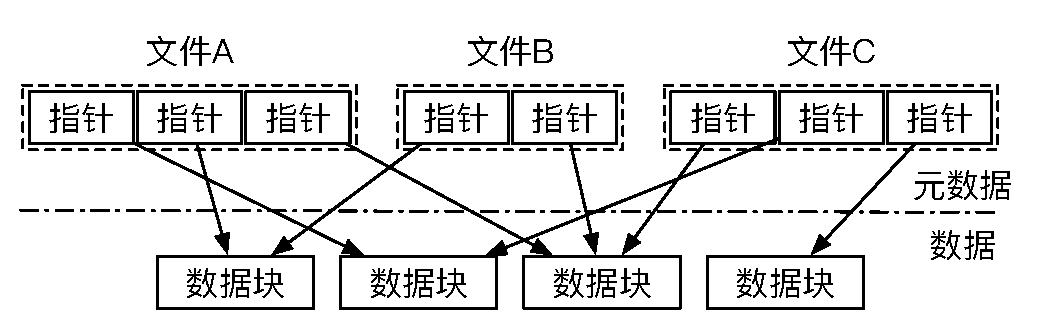
\includegraphics[width=10cm]{DedupSystemStorageMode}
    \caption{数据重删系统的存储模式} 
    \label{fig:数据重删系统的存储模式}
\end{figure}

为了保护数据隐私,加密重复数据删除(encrypted deduplication)增加了一层作用于逻辑数据块的加密操作。如图\ref{fig:加密重复数据删除系统逻辑视图}所示,该加密层基于数据内容来产生加密密钥\citing{bellare2013message}(例如将数据块的哈希值作为密钥\citing{douceur2002reclaiming}),从而将相同的明文数据块加密为相同的密文数据块。系统计算每个密文数据块的哈希值(称为指纹,fingerprint),查询指纹索引(fingerprint index)确定该数据块是否已经存储,最后保存仅具有唯一指纹的密文数据块。需要指出的是,部分加密重复数据删除方案\citing{bellare2013message}采用随机加密算法,但基于明文数据块产生指纹,因此仍然可以通过检查指纹来识别重复数据。

\begin{figure}[!htb]
    \small
    \centering
    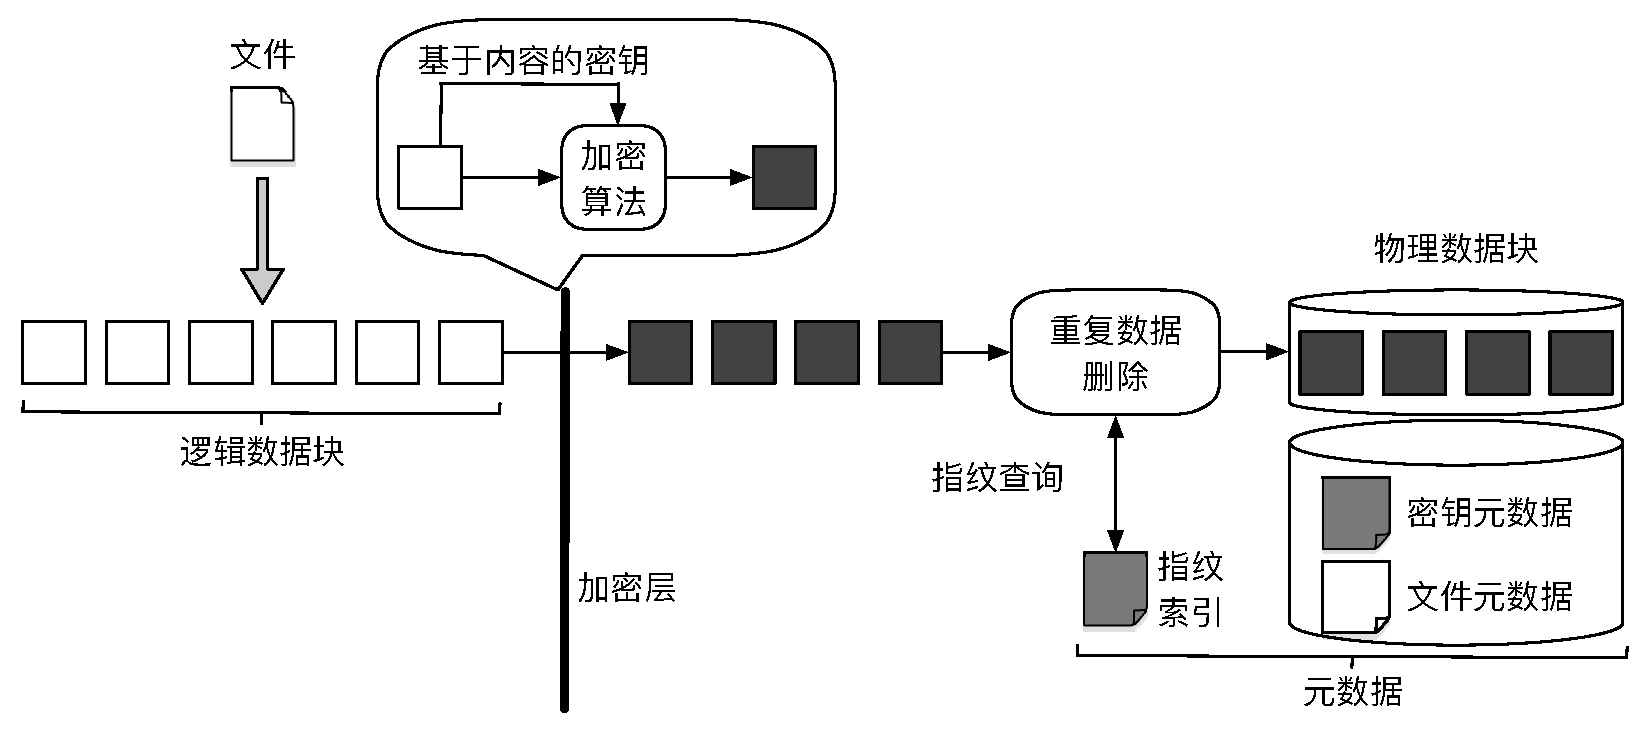
\includegraphics[width=14cm]{EncryptDedupSystemLogic}
    \caption{加密重复数据删除系统逻辑视图}
    \label{fig:加密重复数据删除系统逻辑视图}
\end{figure}

除了指纹索引以外,加密重复数据删除系统须存储额外的元数据(metadata),包括:
\begin{enumerate}
    \item 文件元数据记录了文件内逻辑数据块与相应物理数据块的映射关系,用于重构完整文件。
    \item 密钥元数据记录了文件内逻辑数据块的解密密钥,用于恢复相应的明文内容,由于密钥元数据包含密钥信息,需由文件属主的主密钥(master key)加密后以密文形式存储。
\end{enumerate}

\subsection{问题和动机}

\textbf{数据块频率泄漏问题}

由于基于数据块内容产生密钥,加密重复数据删除泄漏了数据块的频率信息,即如果一个明文数据块出现了n次,则它对应的密文数据块也将出现n次。另一方面,真实数据集中数据块的出现频率往往呈非均匀分布,本文调研了FSL和VM备份数据集(数据集信息见§3.2)的数据块频率分布特征,发现三种数据集有超过97\%的数据块的频率低于100次,而至多只有0.04\%的数据块的频率高于10,000次(图\ref{fig:两种真实数据集的数据块频率分布}),这种非均匀的分布特点使攻击者可以利用频率来确定相应数据块。

基于以上原因,认为加密重复数据删除可能受到频率分析\citing{naveed2015inference}的威胁,拟通过本课题,深入研究频率分析攻击对加密重复数据删除安全性的影响,以及提高频率分析攻击效果的方法。


\begin{figure}[!htb]
    \small
    \centering
    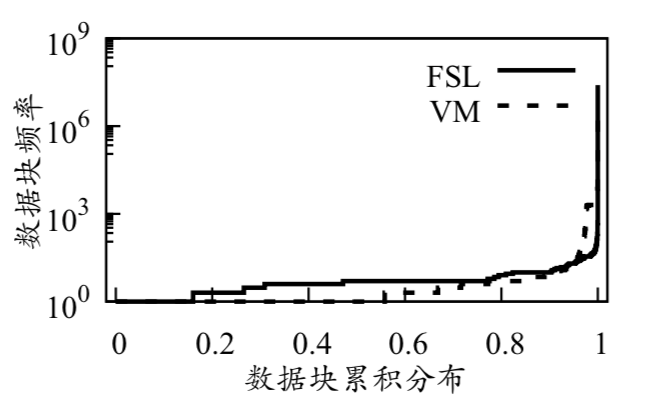
\includegraphics[width=8cm]{两种真实数据集的数据块频率分布.png} %{FSLandVMfrequencyDis.eps} %{两种真实数据集的数据块频率分布.png}
    \caption{两种真实数据集的数据块频率分布} 
    \label{fig:两种真实数据集的数据块频率分布}
\end{figure}

\subsection{研究意义}

本课题研究将填补频率分析攻击研究空白,对理解加密重复数据删除的实际安全性,并降低其在非适合场景下的误用风险具有重要作用。

尽管加密重复数据删除的频率泄漏已是学术界公认的安全问题,但针对性的频率分析攻击研究仍为空白(即利用频率泄漏来获取隐私数据仍是一个开放性问题),致使部分厂商盲目地将加密重复数据删除技术应用于商业产品\citing{MEGA,ElephantDrive}和开源系统\citing{Cryptosphere,Freenet,GNUP2P,Tahoe-LAFS}中。本项目将研究加密重复数据删除技术在频率分析攻击下的实际安全性,以指导其在适合场景下被正确使用。


\section{国内外研究历史与现状}

\subsection{加密重复数据删除}
\label{sec:加密重复数据删除}
在传统对称加密方式下,每个用户具有不同的密钥,不同用户之间的相同明文会被加密为不同密文,难以执行(密文)重复数据删除操作。

消息锁定加密(message-locked encryption,MLE)确立了加密重复数据删除的密码学基础\citing{bellare2013message}:基于数据内容产生密钥(称为 MLE 密钥),从而将相同明文加密为相同密文。最流行的MLE实例是收敛加密(convergent encryption,CE)\citing{douceur2002reclaiming},它使用明文的哈希值作为MLE密钥,并基于密文哈希值计算指纹,以识别重复数据(如图\ref{fig:加密重复数据删除系统逻辑视图})。基于CE的加密重复数据删除方案还包括:

\begin{enumerate}
    \item 哈希收敛加密(hash convergent encryption,HCE)\citing{douceur2002reclaiming}与CE具有相同的MLE密钥产生规则,但基于明文哈希值计算指纹。
    \item 随机收敛加密(random convergent encryption,RCE)\citing{douceur2002reclaiming}使用随机密钥加密以产生非确定的密文,同时也基于明文哈希值来进行重复检查。
    \item 收敛扩散(convergent dispersal,CD)\citing{li2016cdstore}使用明文哈希值作为秘密共享(secret sharing)的输入种子,在兼容重复数据删除的基础上 提高了密文存储的可靠性。
\end{enumerate}

上述MLE实例基于明文产生MLE密钥(CE、HCE和CD)或指纹(HCE和RCE),如果明文是可预测的(即所有可能的明文的数量有限),这些方案易于受到离线暴力破解攻击\citing{bellare2013message,keelveedhi2013dupless}。为了抵御该攻击,DupLESS\citing{keelveedhi2013dupless}基于第三方密钥服务器实现了服务器辅助 MLE(server-aided MLE),确保无法从离线明文派生出相应的MLE密钥。以服务器辅助MLE为基础,现有研究进一步解决了加密重复数据删除的故障容错\citing{li2015cdstore,duan2014distributed}、透明价格模型\citing{armknecht2015transparent}、点对点密钥管理\citing{liu2015secure}、层次密钥管理\citing{zhou2015secdep}等问题。围绕MLE扩展功能的一系列研究包括:兼容加密重复数据删除的数据完整性审计协议\citing{li2016secure};支持动态访问控制的加密重复数据删除系统REED\citing{li2016rekeying,qin2017design}。

无论是MLE还是服务器辅助MLE,均须为相同的明文产生相同的密文(CE、HCE、CD和DupLESS)或指纹(HCE和RCE),泄漏了数据的出现频率。一些理论研究\citing{abadi2013message,stanek2014secure,bellare2015interactive}基于零知识证明、全同态加密、双线性对运算等底层密码技术实现了随机加密,但这些方案存在计算复杂性高、依赖多轮信息交互等问题,难以应用到系统实践中。本文关注可实际应用的加密重复数据删除系统/方案的频率泄漏问题,研究其安全性影响和防御对策。

\subsection{频率分析攻击}
\label{sec:传统频率分析攻击}

频率分析\citing{katz1996handbook}是一种针对确定性加密(deterministic encryption)的密码分析技术,被应用于破解匿名查询日志\citing{kumar2007anonymizing}、破坏关键词隐私\citing{cash2015leakage,grubbs2016breaking,islam2012access,pouliot2016shadow,zhang2016all}、重构密文数据库记录\citing{naveed2015inference,bindschaedler2018tao,durak2016else,grubbs2017leakage,kellaris2016generic,lacharite2018improved} 等实际攻击。本项目研究针对数据块的频率分析攻击,与现有攻击目标(查询日志条目、关键词、数据库记录等)相比,数据块数量极其庞大(呈千万级),并且大量数据块具有相同频率,致使当前的频率分析攻击算法难以适用。

面向加密重复数据删除,已有工作\citing{li2017information}提出了基于数据块局部性(chunk locality)\citing{zhu2008avoiding,lillibridge2009sparse,xia2011silo}的频率分析攻击。本课题的部分技术路线就是在该工作\citing{li2017information}的基础上提出来的,并进一步研究频率分析攻击的准确率和依赖条件,以及面向真实系统的攻击原型。除了频率分析和暴力破解(参见\ref{sec:加密重复数据删除})之外,加密重复数据删除还可能遭受边信道攻击\citing{harnik2010side,halevi2011proofs,mulazzani2011dark}、副本伪造攻击\citing{bellare2013message}、基于数据块长度的攻击\citing{ritzdorf2016information}等威胁,但这些攻击可通过所有权证明\citing{halevi2011proofs}、守卫解密(guarded decryption)\citing{bellare2013message}、固定长度分块等措施进行防御,而本文所研究的频率分析攻击超出了现有保护措施的防御范畴。
%(参见\ref{sec:技术路线})
\section{课题的研究内容、研究目标、以及拟解决的关键问题}
\subsection{研究内容}

\subsubsection*{加密重复数据删除的频率分析攻击}

在传统频率分析模式下,攻击者能够访问明文逻辑数据块集合M和密文逻辑数据块集合$C$($M$和$C$包含重复的明文和密文数据块)。攻击者根据出现频率分别对$M$和$C$中的数据块进行排序,然后将$C$中的密文数据块映射为$M$中与其具有相同排名的明文数据块。但是,传统频率分析在加密重复数据删除中难以形成有效的攻击,主要原因是:$M$和$C$的原始内容可能存在差异(例如$M$和$C$来源于同一个文件系统在不同时间点的备份镜像),将打乱数据块频率排序的对应关系;并且,在频率排序过程中可能存在大量明文和密文数据块具有相同的频率,频率分析难以排序这些数据块来形成正确的对应关系。

为了提高传统频率分析的攻击效果,首先研究基于数据特征的新型频率分析攻击技术。然后,分别从抵抗频率排序干扰和降低攻击发生条件两方面改进攻击技术。最后,实现针对真实系统的频率分析攻击原型,并分析该攻击对各类数据安全性的影响。


\subsection{研究目标}

针对以上研究内容,预期实现如下研究目标: 
\begin{enumerate}
    \item 在理论上,构造针对加密重复数据删除的频率分析攻击,揭示实践中的安全隐患。
    \item 在技术上,以理论研究为支撑,设计并实现针对加密重复数据删除系统/方案的频率分析攻击工具,并在真实系统中进行理论验证和攻击效果测试。 
\end{enumerate}


\subsection{拟解决的关键问题}

本课题致力于解决传统频率分析攻击方法在针对加密重复数据删除方案/系统进行攻击时难以解决的如下问题:

\begin{enumerate}
    \item 明密文数据块的的原始内容可能存在差异(例如一组明密文集合分别来源于同一个文件系统在不同时间点的备份镜像),将打乱数据块频率排序的对应关系。
    \item 在频率排序过程中可能存在大量明文和密文数据块具有相同的频率,基本频率分析攻击难以排序这些数据块来形成正确的对应关系。
\end{enumerate}



%\section{拟采取的研究方案}
%\label{sec:技术路线}
%
%
%
%如图\ref{fig:技术路线图}所示,在支撑研究(基于数据块局部性的频率分析攻击方案\citing{li2017information})的基础上,根据相对频率分布特性,设计抗排序干扰的攻击方法;在数据相似性的基础上,设计低依赖条件的攻击方法。最终设计出针对加密重复数据删除方案/系统的新型频率分析攻击方法及对应的原型软件工具。
%
%\begin{figure}[!htb]
%    \small
%    \centering
%    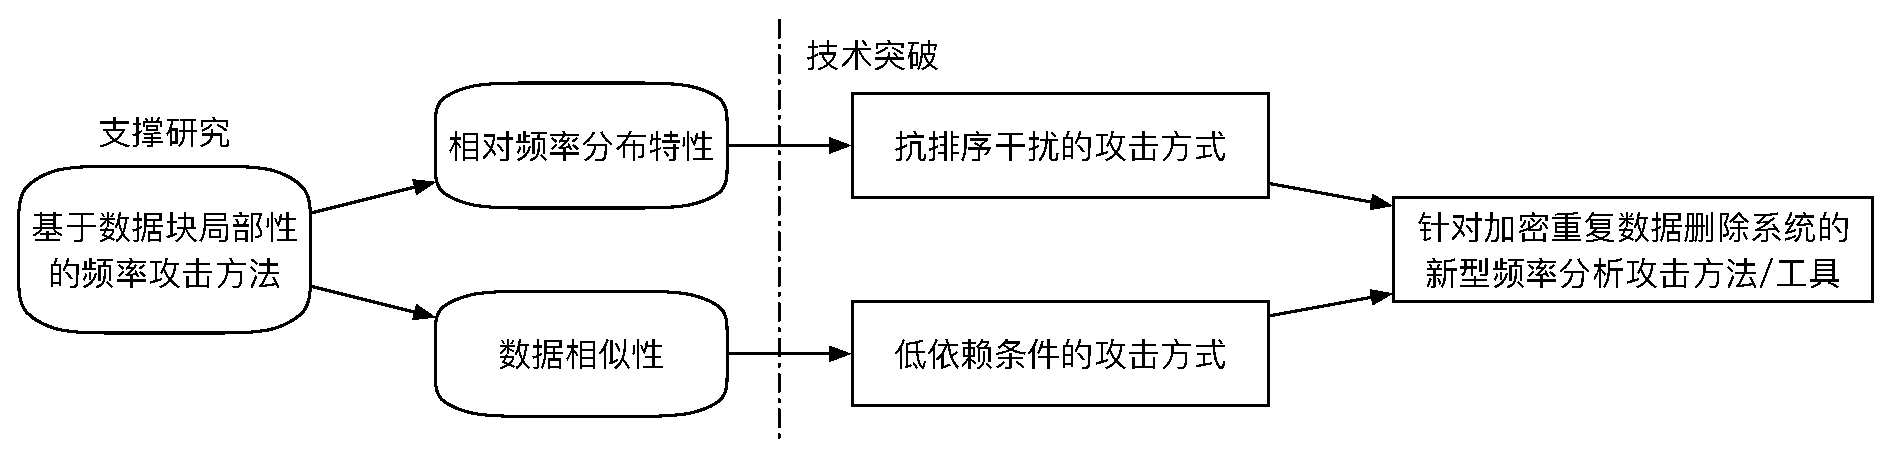
\includegraphics[width=15cm]{TechnicalRoute.eps}
%    \caption{技术路线图} 
%    \label{fig:技术路线图}
%\end{figure}
%
%\subsection{支撑研究}
%
%基于数据块局部性的频率分析攻击方案(locality-based attack)\citing{li2017information}作为支撑研究,该方案主要用于破译加密数据备份,即已知的明文数据块集合$M$和目标密文数据块集合$C$源于同一个系统在两个不同时间点的备份镜像。攻击利用了数据块的局部性特征:在不同备份之间,绝大多数数据块保持了相同的局部顺序;例如,每天备份工作项目的进度快照,若一天内的改动较小,则在两次备份之间未被改动的大部分数据块之间的相对顺序保持不变。因此,得出一个关键推论:如果明文数据块M是密文数据块$C$的原始明文,那么M左边和右边相邻的明文数据块有较大可能也是$C$左边和右边相邻密文数据块的原始明文。
%
%\begin{figure}[!htb]
%    \small
%    \centering
%    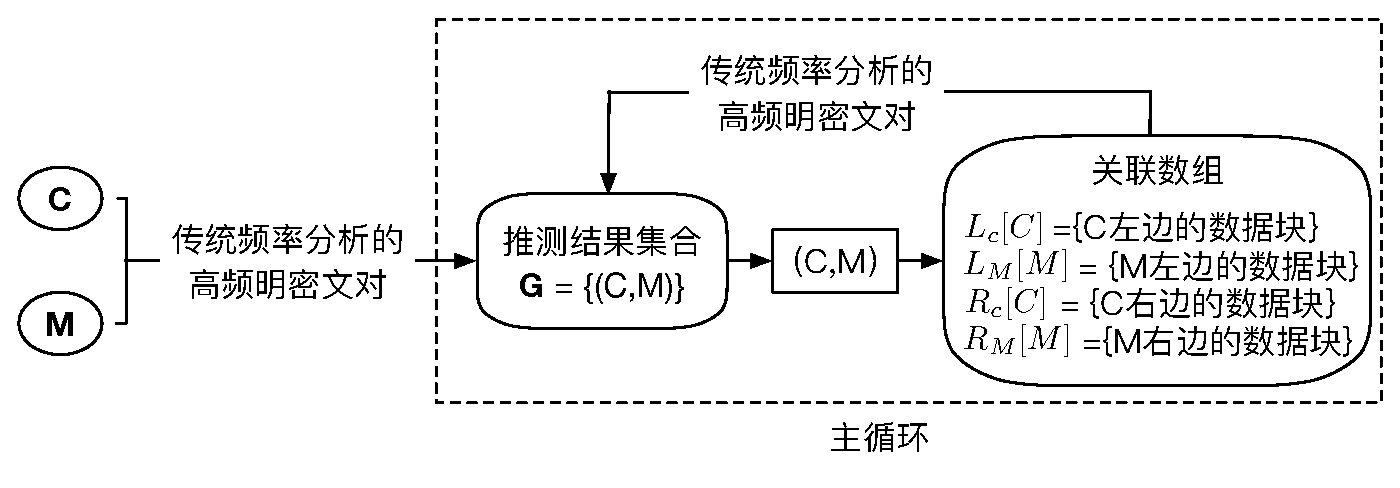
\includegraphics[width=14cm]{BaseFrequencyAttack}
%    \caption{基于数据块局部性的频率分析攻击} 
%    \label{fig:基于数据块局部性的频率分析攻击}
%\end{figure}
%
%
%基于此,攻击流程如图\ref{fig:基于数据块局部性的频率分析攻击}所示:首先,对$C$和$M$应用传统频率分析(参见\ref{sec:传统频率分析攻击}),将获得的若干组高频明密文对加入推测结果集合 $G$;然后,每次从$G$中选取一组明密文对$(M,C)$,分别对其左右相邻的明文和密文数据块集合$L_M[M]$和$L_C[C]$,以及$R_M[M]$和$R_C[C]$实施频率分析,并将获得的高频明密文对也加入$G$;继续对$G$中的明密文对进行基于相邻数据块的频率分析,直至所有明密文对都被处理。
%
%为了验证攻击效果,定义推测率为正确推测出原始明文的(不同)密文数据块个数与$C$中(不同)密文数据块总个数的比率。在基于真实数据集的实验验证中,攻击方案能够达到17.8\%推测率,远远高于传统频率分析方法的0.0001\%推测率。
%
%
%\subsection{技术突破}
%
%\subsubsection{基于分布的频率分析攻击方法}
%
%
%\par 基于分布的频率分析攻击利用密文和明文的相对顺序信息来增强频率分析的有效性。该攻击方法建立在数据块局部性\citing{xia2011silo,lillibridge2009sparse,zhu2008avoiding}的基础上。通过以下三个关键特性构造出基于分布的频率分析攻击方法。
%
%\begin{itemize}
%    \item 数据块局部性指出数据的原始排序可能会在各种备份文件中得以保留,因此可以用于在备份文件中推理出类似的与位置相关的密文-明文对。
%    \item 相邻数据的共现频率的相对频率分布可以通过分析得到。
%    \item 明文及其相应的密文具有相似的相对频率分布的特性。
%\end{itemize}
% 
%\subsubsection{基于聚类的频率分析攻击方法}
%
%
%在基于分布的频率分析攻击方法的基础上,通过引入相似性\citing{bhagwat2009extreme}这一属性来消除基于分布的频率分析攻击方法对明文数据的细粒度顺序信息的需求。基于此提出基于聚类的频率分析攻击方法。
%
%\section{可行性分析}
%
%\subsection{研究方法可行}
%
%本课题通过引入加密重复数据删除方案/系统的相关特性来设计新型频率分析攻击方法,针对性提高频率分析攻击方法的有效性。该研究问题具有很高的实际价值且在面向加密重复数据删除的攻击中,已有工作提出了基于数据块局部性(chunk locality)\citing{zhu2008avoiding,lillibridge2009sparse,xia2011silo}的频率分析攻击\citing{li2017information},在此基础上改进攻击方案以提高频率分析攻击实际效果具有明确的可行性。
%
%\subsection{研究条件可行}
%
%前期基于数据块局部性的频率分析攻击方案给出了本课题研究两种新型频率分析攻击方法的基本理论和工具基础。在原有方案上改进即可用于本课题研究。研究者在本科阶段深入钻研了CDStore、REED、SDFS等加密重复数据删除系统,以及前期基于数据块局部性的频率分析攻击方案的理论和工具实现。这些经验可以帮助设计新型频率分析方法以及其在真实系统中的实践。
%
\section{本文特色与创新之处}

本文的特色与创新之处有以下几点:

\begin{enumerate}
    \item 本文针对加密重复数据删除提出了两种新型的频率分析攻击方法。除了利用由于加密重复数据删除具有确定性导致的频率泄漏之外,两种攻击都利用重复数据删除工作负载的特性来增加频率分析攻击的有效性。
    \item 本文使用多个真实数据集(包括长期备份\citing{sun2016long,FSL14},Windows文件系统快照\citing{meyer2012study}和VM磁盘映像\citing{li2016cdstore,qin2017design})以及开源重复数据删除系统SDFS\citing{SDFS}、Destor\citing{Destor},评估两种新型频率分析攻击方法和基本频率分析攻击方法的实际效果。本文通过评估频率攻击方法的攻击结果,进一步分析本频率分析攻击方法对实际加密重复数据删除带来的安全性影响。
    \item 本文讨论了减少加密重复数据删除中信息泄漏的可能方案。
\end{enumerate}

\section{论文结构及安排}

本文的其余部分安排如下:\ref{sec:background}将介绍本文中将使用的概念的背景知识,\ref{sec:ThreatModel}将介绍本文的威胁模型与假设,\ref{sec:DistributionAttack}将给出本文提出的第一种攻击方法(基于分布的攻击),\ref{sec:ClusteringAttack} 将给出本文提出的第二种攻击方法(基于聚类的攻击),\ref{sec:DataSetSystem}将给出本文实验采用的相关数据来源的介绍, \ref{sec:Experiment}将对两种攻击进行实验分析, \ref{sec:Countermeasure}将给出应对本文提出的攻击方法的一些讨论, \ref{sec:RelatedWork}将介绍重复数据删除与相应攻击的相关工作,最后\ref{sec:Conclusion}对本文进行总结。



\chapter{预备知识}


\chapter{威胁模型}
\label{sec:ThreatModel}
本章为针对加密重复数据删除的频率分析攻击制定了威胁模型。

\section{威胁模型定义}
\label{sec:ThreatModel-Definitions}

本文分别使用$M$和$C$来表示明文数据块(即加密前的逻辑数据块)及其对应的密文数据块(即加密后的逻辑数据块);$|M|$和$|C|$来表示明文数据块(即加密前的逻辑数据块)的大小及其对应的密文数据块(即加密后的逻辑数据块)的大小。

首先将普通文件建模为由$n$个逻辑明文数据块构成的有序列表(即重复数据删除之前的逻辑块),该列表记为$\mathbf{M} = \langle \hat{M}^{(1)}, \hat{M}^{(2)}, \ldots, \hat{M}^{(n)}\rangle$。 每个逻辑明文数据块$\hat{M}^{(i)}$(其中$1\le i\le n$)通过MLE加密得到相应的密文数据块$\hat{C}^{(i)}$。由$\mathbf{M}$的所有加密结果形成由$n$个逻辑密文数据块组成的有序列表记为$\mathbf{C} = \langle \hat{C}^{(1)}, \hat{C}^{(2)}, \ldots, \hat{C}^{(n)} \rangle$。在$\mathbf{C}$中的逻辑密文数据块也会被排序以反映加密重复数据删除存储系统中重复数据删除处理过程的顺序。

相同的逻辑明文和密文可能分别出现在$\mathbf{M}$和$\mathbf{C}$中的不同位置。 本文将一个唯一的明文数据块表示为$M$(通过其指纹的唯一性确定),通过MLE加密得到相应的唯一密文数据块$C$。每个$M$对应于$\hat{M}^{(i)}$的一个或多个相同副本,同理,每个$C$对应于$\hat{C}^{(i)}$的一个或多个相同副本。


\section{对手的目标和相关假设}
\label{sec:ThreatModel-Assumptions}

本文考虑存在一个对手,它准备以以下两个明确的目标为基准推断一组密文数据块-明文数据块对(用\{$(C, M)$\}表示)。


\begin{itemize}
    \item \textbf{推断率高:} 
    
    在所有的正确密文数据块-明文数据块对中,推断出大部分正确的密文数据块-明文数据块对(即统计学上的高召回率或低阴性率)。

    \item \textbf{推断精度高:} 
    
    在所有推断得到的密文数据块-明文数据块对中大部分的密文数据块-明文数据块对的配对是正确的(即统计术语中的高精度或低误报率)。
\end{itemize}
  
  
本文假设该对手是诚实但好奇的,它可以被动地监视密文数据块流$\mathbf{C}$被写入存储系统中的过程,并利用来自$\mathbf{C}$的不同类型的泄漏信息(参见章节:\ref{sec:ThreatModel-Leakage})。鉴于可用的泄漏信息种类,对手仅可通过唯密文攻击的方法推断$\mathbf{C}$中每个密文数据块对应的原始明文数据块。当然,对手也有可能知道有限的密文数据块-明文数据块对的集合来发起已知明文攻击,这种情况进一步加深了攻击的严重性\citing{li2017information}。但在本文中不会考虑前述的已知明文攻击方式。因此,本文将$\mathbf{C}$视为对手所能观察到的的视图,并为该视图的不同属性建模。

本文假设对手无法访问任何包含有关如何操作和存储数据块的信息的元数据(由于不对元数据应用重复数据删除,因此可以通过传统的对称加密来保护这些元数据,这种操作可使得对手无法获知该类型的信息)。此外,本文假设对手没有主动对重复数据删除系统进行攻击的能力,因为这种问题可以通过现有方法予以阻止。例如是恶意客户端可以在客户端重复数据删除中声明对未授权文件拥有所有权\citing{harnik2010side,halevi2011proofs,mulazzani2011dark}; 该问题可以通过所有权证明\citing{halevi2011proofs,xu2013weak,di2012boosting}或服务器端重复数据删除\citing{harnik2010side,li2015cdstore}予以解决。另一个例子是恶意存储系统可以修其改存储的数据;该问题可以通过远程完整性检查来进行检测和解决\citing{juels2007pors,ateniese2007provable}。

\section{三种信息的泄漏}
\label{sec:ThreatModel-Leakage}

本文在加密重复数据删除存储中考虑三种类型的泄漏方式,这些泄漏使得对手能够基于它们推断信息:

\begin{itemize}
    \item \textbf{频率:}  

    由于加密重复数据删除的加密过程的确定性,重复数据删除前$\mathbf{C}$中每个密文数据块的频率(即重复副本数量)可以映射得到$\mathbf{M}$中相应明文数据块的频率。

    \item \textbf{顺序:} 
 
    某些加密重复数据删除存储系统\cite{xia2011silo,lillibridge2009sparse,zhu2008avoiding}为了更高的运行性能,在存储密文数据块是保持了其对应的明文数据块的原始顺序。因此,$\mathbf{C}$中的密文的顺序可以映射到$\mathbf{M}$中的明文的顺序。

    \item \textbf{大小:} 

    可变大小的数据块分块方法(参见章节:\ref{sec:background})产生会产生各种不同大小的明文数据块,如果在对明文数据块进行加密前没有进行数据填充(为了避免增大存储开销\citing{ritzdorf2016information,douceur2002reclaiming,wilcox2008tahoe,keelveedhi2013dupless}),则产生的密文数据块大小与其对应的原始明文数据块大小一致($\mathbf{C}$中的密文大小可以映射到$\mathbf{M}$中相应明文的大小)且密文数据块集合中的密文数据块也具有众多不同的大小。当然,该泄漏可以通过使用块密码算法使得明密文数据块大小不一致来避免。
\end{itemize}

除上述三种泄漏以外,对手还可以获得一些辅助信息,这些信息提供了与$\mathbf{M}$相关的数据特征的基本情况(任何推断攻击都必须提供辅助信息\citing{kumar2007anonymizing,li2017information,grubbs2016breaking,zhang2016all,kellaris2016generic,ritzdorf2016information,naveed2015inference,cash2015leakage,islam2012access})。在这项工作中,将辅助信息视为先前已知的明文数据块(例如,通过旧用户备份或VM磁盘映像得到)构成的有序列表,由$\mathbf{A}$表示。显然,攻击有效性与严重性取决于$\mathbf{A}$(即先前已知的明文数据块)和$\mathbf{M}$(即要推断的明文数据块)之间的相关性。本文的重点不是解决对手如何获取辅助信息的问题。例如,可能是由于粗心的数据发布\citing{careless-release}、被的盗存储设备\citing{stolen-device}和云存储泄漏\citing{cloud-leakage}。相反,根据这些信息,本文研究了可以获得的的辅助信息如何与各种泄漏渠道相结合,给加密重复数据删除带来信息泄漏。

本文将频率分析\citing{al1992origins}作为攻击方法。经典频率分析对$\mathbf{C}$中的唯一密文数据块和$\mathbf{A}$中的唯一明文数据块按频率(即对应于每个唯一密文数据块或唯一明文数据块的相同副本的数量)进行排序。然后,简单的将$\mathbf{C}$中的每个唯一密文数据块与$\mathbf{A}$中具有相同频率等级的唯一明文数据块相关联。基本的频率分析攻击实际效果非常糟糕,在接下来的章节中,本文针对加密重复数据删除设计了较为复杂同时效性极高的频率分析攻击。

\section{本章小结}

本章介绍了针对重复数据删除的威胁模型的定义、本课题研究中将要用到的各种信息来源,以及本文攻击方案的假设的相关说明。






\chapter{基于分布的频率分析攻击方法}
\chapter{基于聚类的频率分析攻击方法}
\label{sec:ClusteringAttack}

本章放松了基于分布的频率分析攻击中的攻击者的攻击条件要求,提出了基于聚类的频率分析攻击,它不需要使用明文数据块的细粒度排序信息。相反,它利用相似性这一属性来推理来自相似的数据段(即,由数据块块聚合形成的更大的数据单元)的原始数据块,而不依赖于每个数据段中的数据块的排序。 本章首先介绍相似性的概念,然后展示如何使该属性进行推理攻击。

\section{背景知识}
\label{sec:similarity}

\subsection{min-wise independence条件}

对于min-wise independence置换族\citing{broder2000min}有如下定义:设$S_n$是$n$元集合$[n]$上所有置换组成的n元对称群。称置换族$F \subseteq S_n$满足min-wise independence条件是指:对任意$X=\{x_1,x_2,\cdots,x_m\}\in[n]$和任意$x_i-inX$,从集合$F$中随机、均匀地选取函数$h$,计算$H(X)=\{h(x_1),h(x_2),\cdots,h(x_m),\}$,有下式成立:
\begin{equation}
    \label{eq:min-wise independence}
    Pr(min(H(X)) = h(x_i) ) = \frac{1}{|X|}
\end{equation}

即$X$中的所有元素在$h$的作用下都有相等的概率成为$H(X)$中的最小元。在实际应用中,完全满足min-wise independence条件的哈希函数很难实现,通常使用近似满足min-wise independence条件\citing{broder2000min}的哈希函数即可。

\subsection{Broder定理}
Broder定理\citing{broder1997resemblance}的定义为:两集合$S_1$和$S_2$,$H(S_i)=\{h(x_k)|\forall x_k \in S_i \}$,h是满足min-wise independence条件的哈希函数,$min(S_i)$代表集合$S_i$中的最小元,则

\begin{equation}
    \label{eq:broder}
    \Pr[\min\{{\rm H}(S_1)\} = \min\{{\rm H}(S_2)\} ] = \frac{|S_1 \cap S_2|}{|S_1 \cup S_2|}
\end{equation}

\subsection{相似性}
相似性\citing{bhagwat2009extreme}指出来自同一来源的备份文件可能类似并且共享大部分相同的数据块。 备份文件之间的相似性可以通过Broder定理\citing{broder1997resemblance}来量化。具体来说,如果将每个文件视为一个数据块的集合$S$(即忽略它们的顺序),Broder定理指出如果两组数据块共享相同的最小数据块哈希值的概率很高,则两个集合包含的数据块可能大部分都相同,反之亦然:
 
\begin{equation}
	\Pr[\min\{{\rm H}(S)\} = \min\{{\rm H}(S')\} ] = \frac{|S \cap S'|}{|S \cup S'|}
	\label{eq:similary}
\end{equation}

其中${\rm H}(\cdot)$是一个从min-wise independence置换族中随机统一选择的哈希函数,$\min\{{\rm H}(S)\}$是$S$的最小数据块的哈希。为了便于描述,本文使用MinHash来表示集合中元素的最小哈希值。


针对重复数据删除的各个方面(性能方面\citing{qin2017design,xia2011silo,bhagwat2009extreme},安全方面\citing{li2017information})的已有工作已经利用了相似性这一属性来保持存储效率。具体来说,它们仅针对共享相同最小数据块哈希的文件(即类似的文件)采用MinHash作为一个数据块集合中所有数据块加密使用的密钥进行重复数据删除。根据Broder定理可以推理得到这类文件可能具有大量相同的数据块,因此这种近似精确的重复数据删除只会导致存储效率的轻微降低。与先前的方法不同\citing{qin2017design,xia2011silo,bhagwat2009extreme,li2017information},本文应用相似性来提高频率分析攻击的有效性。
 
\section{基于聚类的频率分析攻击方法定义}
\label{sec:clustering-attack-description}

现在提出基于聚类的频率分析攻击方法(图:\ref{fig:基于聚类的攻击方法的工作流程}),它基于相似性在加密重复数据删除中推理密文数据块的原始明文数据块。

\begin{figure}[!htb]
    \small
    \centering
    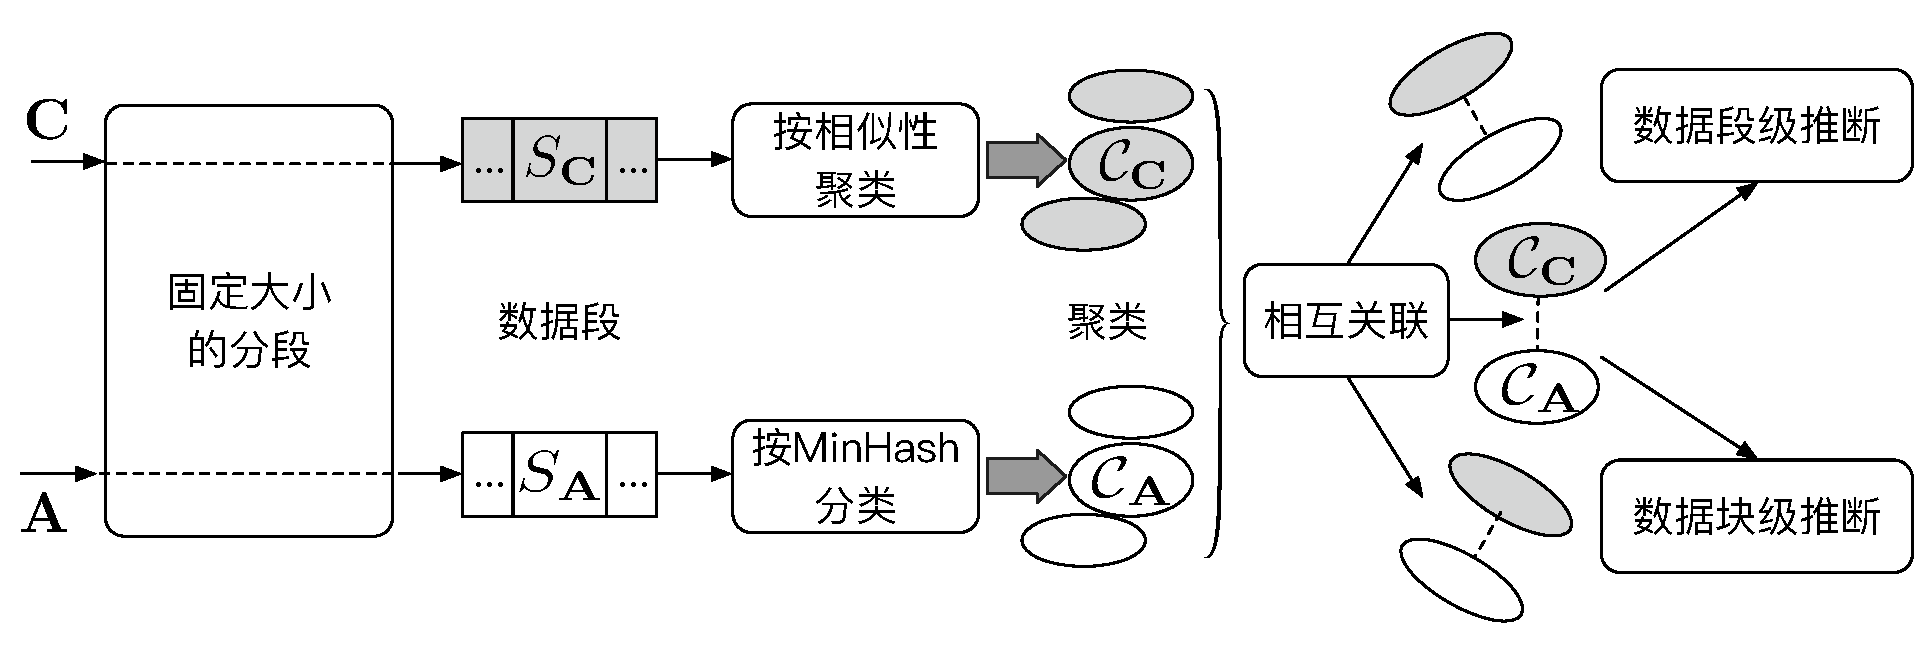
\includegraphics[width=14cm]{ClusteringAttack.eps}
    \caption{基于聚类的攻击方法的工作流程:用MinHash表示明文数据段的最小块散列} 
    \label{fig:基于聚类的攻击方法的工作流程}
\end{figure}

为了利用相似,本文首先在数据块概念的基础上引入数据段的概念。具体来说,将$\mathbf{C}$划分为为一些粗粒度的数据单元,成为密文数据段。密文数据段使用$S_\mathbf{C}$来表示,其中包含有$\mathbf{C}$中的多个相邻的密文数据块。在本课题中,应用了定长分段方法,以确保每个数据段具有相同分的大小(例如,默认大小为4MB)。同样的,对于攻击者所具有的辅助信息$\mathbf{A}$,也同样使用定长分段方法产生多个明文数据段,每个数据段由$S_\mathbf{A}$表示。

注意,一些可变大小的分段方案\citing{lillibridge2009sparse,qin2017design}在其内容与特定模式匹配的数据块之后设置分段边界,从而解决固定大小分段方案所面临的边界移位问题。但是,本文不能在攻击中使用这些可变大小的分段方案\citing{lillibridge2009sparse,qin2017design}。其原因是密文数据段中的数据块的原始内容受到对称加密的保护,攻击者无法确保密文和明文数据段的边界匹配采用的是相同的模式。该问题会导致密文和明文数据段不兼容,从而会降低基于聚类的攻击方法所推理的数据段级的数据量(请参阅本章后半部分)。
 
本方法通过类似的数据段来推理密文-明文对。给出$S_\mathbf{M}$是对应于密文数据段$S_\mathbf{C}$的明文数据段(即$S_\mathbf{M}$中的每个明文数据块对应于$S_\mathbf{C}$中的某些密文数据块,反之亦然)。根据Broder定理,如果一个明文数据段$S_\mathbf{M}$与辅助信息中的明文数据段$S_\mathbf{A}$具有相同的最小数据块哈希(称为$h$),则$S_\mathbf{M}$和$S_\mathbf{A}$可能拥有拥有大量相同的明文数据块。这意味着$S_\mathbf{C}$中的密文数据块很可能是从$S_\mathbf{A}$中的明文数据块映射得到的。换言之,攻击者首先按照最小数据块哈希对$\mathbf{A}$中的所有明文数据段进行分类,以此获得多个明文数据段集合(聚类的不同类别)。将每个明文数据段集合用$\mathcal{C}_\mathbf{A} = \{ S_\mathbf{A} \}$表示,对应于该集合中包含的所有明文数据段共有的唯一最小数据块哈希。同理,攻击者将密文数据段也进行上述分类操作,对于每个分类的集合用$\mathcal{C}_\mathbf{C} = \{ S_\mathbf{C} \}$表示)。然后,攻击者从对应于某一最小数据块哈希$h$的$\mathcal{C}_\mathbf{A}$中推理出$\mathcal{C}_\mathbf{C}$的原始明文数据。  

在本文中,定义任意两个密文数据段$S_\mathbf{C}$和$S_\mathbf{C}'$的聚类距离$d(S_\mathbf{C},S_\mathbf{C}')$为1减去相同密文的分数:

\begin{equation}
\label{eq:distence}
    d(S_\mathbf{C}, S_\mathbf{C}') = 1 - \frac{|S_\mathbf{C} \cap S_\mathbf{C}'|}{|S_\mathbf{C} \cup S_\mathbf{C}'|}.
\end{equation}

在推理过程中,相同的密文可能会在$S_\mathbf{C}$或$S_\mathbf{C}'$中重复出现,而$|S_\mathbf{C} \cap S_\mathbf{C}'|$和$|S_\mathbf{C} \cup S_\mathbf{C}'|$ 会分别返回其交集和并集中具有唯一性的密文数据块的数量。显然,$d(S_\mathbf{C}, S_\mathbf{C}')$越小,则说明$S_\mathbf{C}$和$S_\mathbf{C}'$更可能对应相同的最小数据块哈希。在本章中,采用凝聚法层次聚类(AHC)\citing{johnson1967hierarchical}方法来根据距离信息聚合相似的密文数据段。具体来说,攻击者从其拥有的每个密文数据段开始,将每个密文数据段视为一个单独的聚类类别,然后计算各个聚类之间的距离,将两个距离最近的(最相似的)聚类合并在一起,不断迭代这一过程直到任意两个聚类间的距离均大于给定最大距离参数$k$时停止迭代操作。
 
对于最终得到的每个密文聚类$\mathcal{C}_\mathbf{C}$,攻击者在考虑频率分布的前提下通过频率分析将其与一些明文聚类$\mathcal{C}_\mathbf{A}$相关联。该操作方法基于如下观察:相同的密文数据段(明文数据段)可以在相同或不同的密文数据段(明文数据段)中重复出现,并且相同的密文(明文)数据段也可以在相同的密文(明文)聚类中重复出现。同时,攻击者检查每个聚类中明文数据块或密文数据块的频率分布,并且认为相似的聚类(即,对应于相同的最小数据块哈希)中数据块的频率分布也是相似的。
 
本文按如下的顺序来设计频率分析攻击方案。首先,将所有可用的密文和明文聚类分别按它们包含的逻辑密文数据块和明文数据块的总数进行排序。然后,计算一个关联数组$\mathbf{F}$用于存储相应聚类中每个具有唯一性的密文数据块或明文数据块的频率。基于 $\mathbf{F}$,计算密文数据块$C$存在于密文聚类$\mathcal{C}_\mathbf{C}$中的概率$\Pr[C \in \mathcal{C}_\mathbf{C}]$,并进一步计算$\mathcal{C}_\mathbf{C}$的熵$e(\mathcal{C}_\mathbf{C})$:     

\begin{equation}
\begin{aligned}
\label{eq:Pr&eincluster}
    \Pr[C \in \mathcal{C}_\mathbf{C}] &= \frac{\mathbf{F}[\mathcal{C}_\mathbf{C}][C]}{\sum_{C' \in \mathcal{C}_\mathbf{C}} \mathbf{F}[\mathcal{C}_\mathbf{C}][C']} \\
    e(\mathcal{C}_\mathbf{C}) &= \sum_{C \in \mathcal{C}_\mathbf{C}} \log_2 \frac{1}{\Pr[C \in \mathcal{C}_\mathbf{C}]} 
\end{aligned}
\end{equation}

其中$\mathbf{F}[\mathcal{C}_\mathbf{C}][C]$存储了$\mathcal{C}_\mathbf{C}$中密文数据块$C$的频率。同理,计算出明文聚类$\mathcal{C}_\mathbf{A}$的熵$e(\mathcal{C}_\mathbf{A})$。与基于分布的频率分析攻击(参见\ref{sec:distribution-attack-description})类似,本文使用参数$(u, r, t)$来配置频率分析攻击方案。如果密文聚类$\mathcal{C}_\mathbf{C}$和明文聚类$\mathcal{C}_\mathbf{A}$满足如下三个条件则可说明两个聚类相似:   


\begin{itemize}
    \item  $\mathcal{C}_\mathbf{C}$的排名数值大小不大于$u$。
    \item  $\mathcal{C}_\mathbf{C}$和$\mathcal{C}_\mathbf{A}$的排名数值差距大小不大于$r$。  
    \item  $e(\mathcal{C}_\mathbf{C})$和$e(\mathcal{C}_\mathbf{A})$的差异是最小的,且不超过$t$.
\end{itemize}

然后,对于每个相似的聚类对$(\mathcal{C}_\mathbf{C}, \mathcal{C}_\mathbf{A})$,攻击者在两个级别分别进行明密文对的推理工作。

\begin{itemize}
    \item \textbf{数据段级推理}
    
    \par 如果$\mathcal{C}_\mathbf{C}$和$\mathcal{C}_\mathbf{A}$拥有相同数量的逻辑数据块(即密文数据块或明文数据块)以及相同的熵,则$\mathcal{C}_\mathbf{C}$与$\mathcal{C}_\mathbf{A}$完全映射的概率很高。在这种情况下,攻击者对粗粒度的数据段进行攻击。具体来说,攻击者首先在$\mathcal{C}_\mathbf{C}$中基于其密文的频率分布计算每个密文数据段$S_\mathbf{C}$的熵,并在$\mathcal{C}_\mathbf{A}$中基于其明文的频率分布计算每个明文数据段$S_\mathbf{A}$的熵。
         
         
    \par 如果$S_\mathbf{C}$和$S_\mathbf{A}$中逻辑数据块的总数和熵一致,则攻击者可以推理密文数据段$S_\mathbf{C}$是由命文数据段$S_\mathbf{A}$映射得到的。根据实验表明,基于聚类的频率分析攻击中大部分推理正确的内容来自于数据段级推理。同时,攻击者还可以利用额外的对抗性知识(例如,逻辑块顺序)来进一步恢复这些推理出的数据段中的每个数据块的明文。
         
    \item \textbf{数据块级推理}
    
    
    \par 如果$\mathcal{C}_\mathbf{C}$和$\mathcal{C}_\mathbf{A}$中具有的逻辑块数量或熵不同,攻击者对细粒度的数据块进行攻击。具体来说,攻击者分别对$\mathcal{C}_\mathbf{C}$和$\mathcal{C}_\mathbf{A}$中的具有唯一性的密文数据块和明文数据块按照出现频率进行排序,以此根据频率排名的顺序推理明文数据块-密文数据块对。            
     
    \par 然而,实验发现数据块级推理在本文给出的实验数据集中表现不佳。可能的原因是每个聚类包括大量逻辑数据块,这降低了频率分析的有效性。但即便如此,本文预计数据块级推理可以在实践中正确推理出更多的密文数据块-明文数据块对,当某些聚类中的逻辑数据块数量有限时效果会更佳。
 
\end{itemize}

\subsection{基于聚类的频率分析攻击方法总结}

总而言之,基于聚类的频率分析攻击利用相似性,在类似的聚类类别中使用频率分析攻击以推理密文数据块-明文数据块对。 除$u$,$r$和$t$外,它还由参数$k$配置,该参数指定了配对两个聚类类别的距离上限。

尽管可能受到固定大小数据段的边界偏移问题的影响,但本文认为基于聚类的频率分析攻击对VM磁盘映像的攻击效果是显著的。VM映像文件在创建时被分配了固定的大小,并且在其生存期内无法改变。在开始写入数据前,VM映像中的所有空间均由全零数据进行填充。在将数据存入映像的过程中,通过将需要用到的部分空间进行重写来完成数据存入过程。在章节\ref{sec:experiment-clustering}中,本文研究了针对VM磁盘映像的基于聚类的频率分析攻击的有效性。

\section{本章小结}

本章介绍了本文提出的第二种改进的频率分析方法:基于聚类的频率分析攻击方法。给出了该方法的相关背景知识、形式定义、方法描述以及最佳的适用场景。                  



\chapter{数据集与实际系统调研}
\section{数据集}
\subsection{FSL数据集}
\subsection{VM数据集}
\subsection{MS数据集}

\section{实际系统}
\subsection{SDFS}

\subsection{Destor}

\chapter{实验测试与分析}
\label{sec:Experiment}

In this section, we present the trace-driven evaluation results to demonstrate
the severity of our proposed frequency analysis attacks against encrypted
deduplication.

\section{Methodology}
\label{sec:dataset}

\begin{table}[!t]
    \caption{Characteristics of experimental datasets.}
\small
\label{tab:dataset}
\renewcommand{\arraystretch}{1.2}
\vspace{-3pt}
\centering
\begin{tabular}{|c|c|c|c|}
\hline
 \multirow{2}{*}{\bf Dataset} & \multirow{2}{*}{\bf Category} & \multicolumn{2}{c|}{\bf Characteristics in Each Snapshot} \\
\cline{3-4}
    & &  \#Logical (Million) & \#Unique (Million) \\
\hline
    \multirow{6}{*}{FSL} & User004  & 1.0-1.3 & 0.7-0.9\\
 \cline{2-4}
              & User007 &  3.5-5.2 & 2.3-3.6 \\
 \cline{2-4}
              & User012 &  25.0-26.4 & 8.9-9.7 \\
\cline{2-4}
              & User013 &  1.8-5.7 & 1.2-4.2 \\
\cline{2-4}
              & User015 &  13.4-20.5 & 9.0-11.0 \\
\cline{2-4}
              & User028 &  6.0-10.3 & 3.5-6.8 \\
\hline
\hline
    \multirow{4}{*}{MS} & Win7  & 61.6-61.8 & 61.1-61.3\\
\cline{2-4}
              & Serv-03 & 10.6-10.7 & 8.4-8.5\\
\cline{2-4}
              & Serv-08 & $\sim$6.5 & $\sim$3.8 \\
\cline{2-4}
              & Vista-B &  $\sim$7.6 & $\sim$2.0\\
\cline{2-4}
              & Vista-U &  $\sim$21.0 & $\sim$10.4 \\
\hline
\hline

    \multirow{6}{*}{VM} & User1  &  \multirow{6}{*}{2.6} & $\sim$0.9 \\
\cline{2-2}
\cline{4-4}
              & User2 &  & 1.1-1.3 \\
\cline{2-2}
\cline{4-4}
              & User3 &  & 0.9-1.1 \\
\cline{2-2}
\cline{4-4}
              & User4 &  & $\sim$0.9 \\
\cline{2-2}
\cline{4-4}
              & User5 &  & 0.9-1.0 \\
\cline{2-2}
\cline{4-4}
              & User6 &  & 0.9-1.1 \\
\hline
\end{tabular}
\medskip

\raggedright
    The notations \#Logical and \#Unique denote the total number of logical and unique chunks in each experimental snapshot, respectively. 
    % All VM images have a fixed size of 10GB and hence the same number of logical chunks.
\end{table}



%\begin{table}[!t]
%\small
%\caption{Experimental datasets.}
%\label{tab:dataset}
%\renewcommand{\arraystretch}{1.2}
%\vspace{-3pt}
%\centering
%\begin{tabular}{|c|c|c|}
%\hline
%{\bf Dataset} & {\bf Category} & {\bf Approximate Logical Size} \\
%\hline
%\hline
%%\multirow{2}{*}{FSL} & Physical  & 431.9GB  & 659.3GB & 584.3GB \\
%	\multirow{6}{*}{FSL} & User004  & 10GB/backup $\times$ 14 backups \\
%\cline{2-3}
%			  & User007 & 39GB/backup $\times$ 14 backups \\
%\cline{2-3}
%			  & User012 & 244GB/backup $\times$ 14 backups \\
%\cline{2-3}
%			  & User013 & 22GB/backup $\times$ 14 backups\\
%\cline{2-3}
%			  & User015 & 158GB/backup $\times$ 14 backups\\
%\cline{2-3}
%			  & User028 & 77GB/backup $\times$ 14 backups\\
%\hline
%\hline
%\multirow{4}{*}{MS} & WIN7  & 425GB/snapshot $\times$ 4 snapshots \\
%\cline{2-3}
%			  & Serv-03 & 78GB/snapshot $\times$ 4 snapshots \\
%\cline{2-3}
%			  & Serv-08 & 48GB/snapshot $\times$ 4 snapshots \\
%\cline{2-3}
%			  & Vista-B & 55GB/snapshot $\times$ 4 snapshots \\
%\cline{2-3}
%			  & Vista-U & 159GB/snapshot $\times$ 4 snapshots \\

%\hline
%\hline

%\multirow{6}{*}{VM} & User1  & 25GB/backup $\times$ 13 backups \\
%\cline{2-3}
%			  & User2 & 28GB/backup $\times$ 13 backups \\
%\cline{2-3}
%			  & User3 & 26GB/backup $\times$ 13 backups \\
%\cline{2-3}
%			  & User4 & 25GB/backup $\times$ 13 backups\\
%\cline{2-3}
%			  & User5 & 25GB/backup $\times$ 13 backups\\
%\cline{2-3}
%			  & User6 & 27GB/backup $\times$ 13 backups\\

%% \multicolumn{2}{|c|}{\bf Storage saving} & 98.6\% & 98.3\% \\
%\hline
%\end{tabular}
%\end{table}
We evaluate our attacks using the following real-world datasets, whose
characteristics are summarized in Table~\ref{tab:dataset}. 
% Table~\ref{tab:dataset} summarizes the characteristics of the experimental datasets used in our experiments. 
% We evaluate our attacks using the following datasets. 
% investigate the security implications of the leakages (see \S\ref{sec:background}) by means of simulated attacks, 

\begin{itemize}[leftmargin=*]
\item 
\textbf{FSL:} This dataset is collected by the File systems and
        Storage Lab (FSL) at Stony Brook University \cite{sun16,FSL14,sun18}. We focus on
the {\em fslhomes} snapshots, each of which includes an ordered list of 48-bit
chunk hashes that are produced by variable-size chunking under an average size
of 8KB, as well as the corresponding metadata information (e.g., chunk size,
file name extension, etc). We pick the snapshots from January 22 to May 21 in
2013, and select six users (i.e., User004, User007, User012, User013, User015,
and User028) that have the complete daily snapshots over the whole duration.
We collect these snapshots on a weekly basis, and hence form 14 weekly full
backups for each user.  
\item 
\textbf{MS:} This dataset is collected by Microsoft
\cite{meyer11} and publicized on SNIA \cite{ms}. The original dataset contains
the Windows file system snapshots that span from September 5 to October 31,
2009. Each snapshot is represented by the 40-bit chunk hashes under different
average sizes obtained from Rabin fingerprinting \cite{rabin81}.  We focus on
the snapshots that have been installed with the operating systems in the
following categories: Windows 7 (Win7), Microsoft Windows Server 2003
(Serv-03), Microsoft Windows Server 2008 (Serv-08), Microsoft Windows Vista
Business Edition (Vista-B), and Microsoft Windows Vista Ultimate Edition
(Vista-U). In each category, we pick four snapshots, each of which is
configured with the average chunk size of 8KB.   
\item 
\textbf{VM:} This dataset is collected from a university programming course in
Spring 2014. The original dataset includes a number of VM image snapshots for
the students enrolled in the course, and each snapshot has a fixed size of
10GB and is represented by the ordered list of SHA-1 hashes of 4KB fixed-size
chunks. We focus on 6 users (i.e., User1-User6) and extract their snapshots
into 13 weekly backups.  
%Prior studies \cite{qin17, li15} have used some variants of the dataset for
%different evaluation purposes, and we aim to validate the severity of the
%clustering-based attack against VM disk images.   
\end{itemize}

Our datasets do not contain actual content, so we mimic the adversarial
knowledge based on chunk hashes. Specifically, we use the ordered lists of
chunk hashes in some snapshots as the auxiliary information $\mathbf{A}$ and
the ground truth $\mathbf{M}$, respectively. To simulate encryption, we apply
an additional hash function over each original chunk hash (that represents a
plaintext) in $\mathbf{M}$, and truncate the result into an agreed number of
bits specific to the used dataset. The truncated result mimics a ciphertext in
$\mathbf{C}$. For each inferred ciphertext-plaintext pair $(C, M)$, we verify
its correctness by applying the same simulated encryption on $M$ and comparing
the result with $C$. Note that the clustering-based attack can operate at the
segment level, and infer the ciphertext-plaintext segment pair $(S_\mathbf{C},
S_\mathbf{A})$.  In this case, we check $(S_\mathbf{C}, S_\mathbf{A})$ by
examining each ciphertext in $S_\mathbf{C}$ is exactly mapped from each
plaintext in $S_\mathbf{A}$.

% , although we cannot recover each chunk in the real attack.   
% We count the leakage (see \S\ref{sec:threat}) of each ciphertext chunk, and use it for our inference attacks.  
% MD5 on each hash (that represents a plaintext) in $\mathbf{M}$, and truncate the resulting hash into an agreed number of bits (e.g., 48-bit for FSL, 40-bit for MS, and 160-bit for VM).  

We measure the severity of the attacks by the inference rate and the inference
precision (see Section~\ref{sec:threat}). 

\section{Results of Distribution-based Attack}
\label{sec:experiment-distribution}

\begin{figure*}[t]
    \centering
    \begin{tabular}{p{.31\textwidth}p{.31\textwidth}p{.31\textwidth}}
        \multicolumn{3}{c}{
\includegraphics[width=.7\textwidth]{pic/legend-fsl-line.pdf}} \smallskip \\
        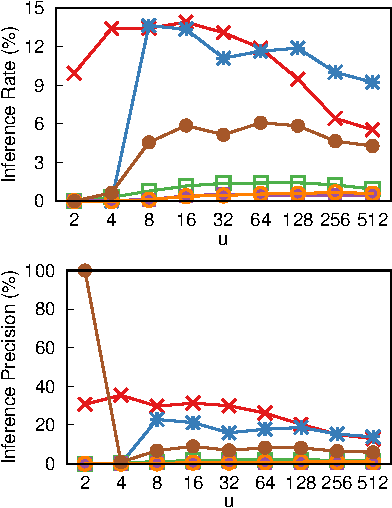
\includegraphics[width=.3\textwidth]{pic/distribution-impact-u.pdf} &
        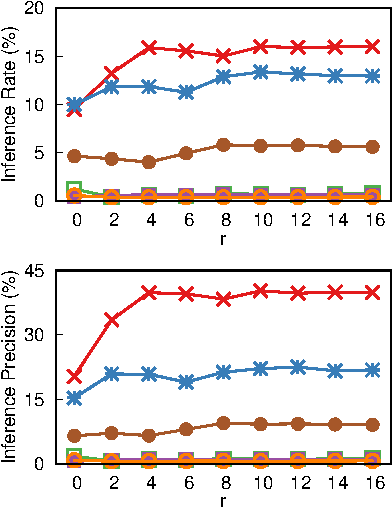
\includegraphics[width=.3\textwidth]{pic/distribution-impact-r.pdf} &
	    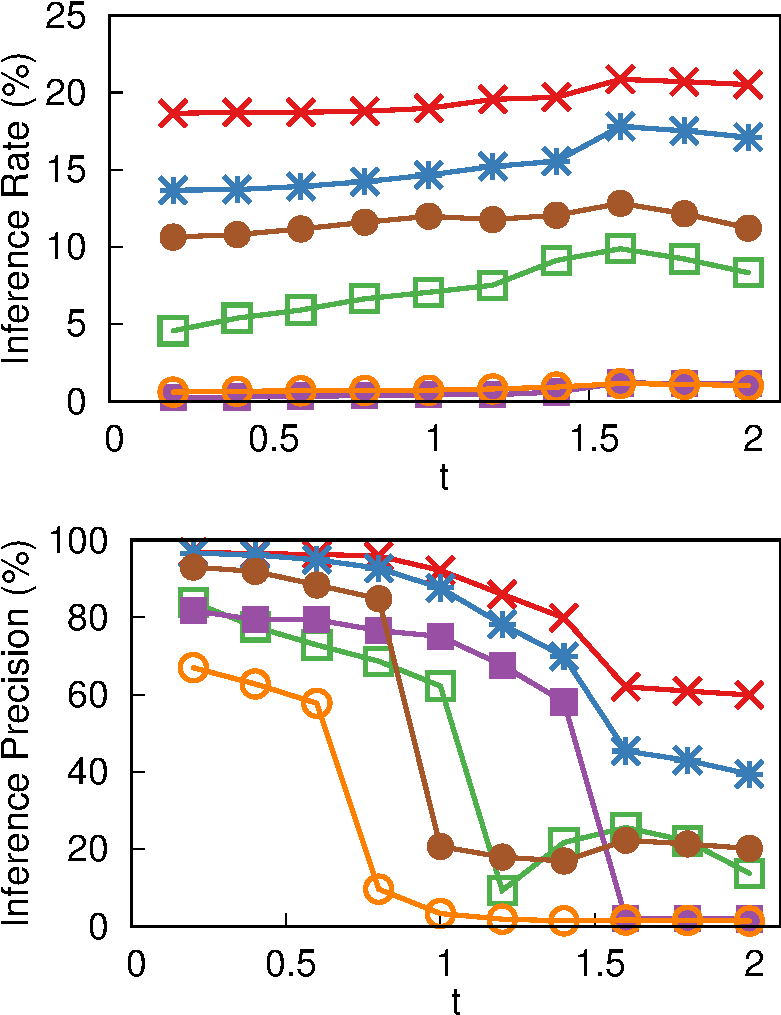
\includegraphics[width=.3\textwidth]{pic/distribution-impact-t.pdf} \medskip \\
        {\footnotesize 
        \centering
        (a) Impact of $u$: $r$ = 0; $t \rightarrow \infty$
        } &
        {\footnotesize
        (b) Impact of $r$: $u$ = 128 for User004, User013 and User015, and $u$ = 256 for User007, User012 and User028; $t \rightarrow \infty$
        } &
        {\footnotesize
        (c) Impact of $t$: $u$ = 128 for User004, User013 and User015, and $u$ = 256 for User007, User012 and User028; $r$ = 10
        } \\
    \end{tabular}
    \caption{Experiment 1 (Impact of parameters): impact of $(u, r, t)$ in distribution-based attack.}
    \label{fig:distribution-impact}
\end{figure*}


\subsection{Experiment 1 (Impact of parameters):}
We evaluate the impact of the parameters $(u, r, t)$ in the distribution-based
attack. We drive our evaluation using the FSL dataset, and use the 12th weekly
backup of each user as the auxiliary information to infer original plaintexts
in corresponding 14th weekly backup.  We configure $t \rightarrow \infty$ and $r$ = 0 to
evaluate the impact of $u$ (in this case, the distribution-based attack
reduces to the locality-based attack \cite{li17}). Our rationale is to avoid
the disturbances by other parameters. 

Figure~\ref{fig:distribution-impact}(a) shows the impact of $u$,
when we vary $u$ from 2 to 512. Regarding inference rate, we have the same
observation as the prior work \cite{li17}. Specifically, the inference rates
first increase with $u$, since the attack can infer more ciphertext-plaintext
pairs. After hitting the maximum values (e.g., 13.9\% for User004, 13.6\% for
User007, 1.4\% for User012, 0.5\% for User013, 0.7\% for User015, and 6.1\%
for User028), they decrease.  The reason is that the underlying frequency
analysis introduces a large number of false positives that compromise the
inferences over corresponding neighbors.    

The prior work \cite{li17} does not report the inference precision about the
attack. We observe that the inference precisions for all users are at a
fairly low level (e.g., less than 40\%), except the case of $u = 2$ for
User028 that does not introduce any false positives. On the other hand, the
inference rate in the special case is about 0.0001\%, meaning that the attack
only infers a few ciphertext-plaintext pairs. In addition, as $u$ increases,
the inference precisions decrease slightly. For example, when $u$ increases
from 2 to 512, the inference precision of User004 drops from 30.7\% to 12.8\%.      

{\bf Observation (1) --} {\em A relatively larger $u$ increases the inference
rate, yet it decreases the inference precision (i.e., more false positives are
introduced). }

Informed by the impact of $u$, we set $u$ at 128 for User004, User013 and
User015, and at 256 for User007, User012 and User028, respectively, in order
to evaluate the impact of $r$ and $t$. 
% {\bf Note that the configuration
% exceeds the best one that leads to the highest inference rate. PC: I don't
% quite understand???} 
Our rationale is to increase the coverage of inferred ciphertext-plaintext
pairs, while we use $r$ and $t$ to filter possibly false positives. 

We first configure $t \rightarrow \infty$ and evaluate the impact of $r$. Figure~\ref{fig:distribution-impact}(b) shows the results. We observe that the
inference rates of majority users increase with $r$. For example, when we vary
$r$ from 0 to 16, the inference rates grow from 9.5\% to 16.0\%, from 10.0\%
to 13.0\%, from 0.5\% to 0.7\%, and from 4.7\% to 5.6\% for User004, User007,
User013, and User028, respectively. The reason is that the distribution-based
attack addresses disturbances to frequency ranking, and infer more correct
ciphertext-plaintext  pairs. On the other hand, the inference rates decrease
slightly from 1.3\% to 0.8\% and from 0.6\% to 0.4\% for User012 and User015,
respectively. The reason is that they examine a large range of plaintexts and
may introduce more false positives. In addition, the inference precisions for
all users are  at a low level (e.g., less than 45\%), and have similar
tendencies with corresponding inference rates.  

{\bf Observation (2) --} {\em A larger $r$ provides more opportunities of
identifying correct ciphertext-plaintext pairs, yet it also increases the
probability of having false positives.}   

Then, we fix $r$ = 10 and evaluate the impact of $t$. 
Figure~\ref{fig:distribution-impact}(c) shows the results. When $t$ is small
(e.g., less than 0.5), we observe that the attack misjudges and filters a
significant number of ciphertext-plaintext pairs, even they are correct. This
introduces {\em false negatives} that reduce the inference rate. As $t$
increases, the number of false negatives decreases.  When $t$ = 1.5, the
inference rates hit the maximum values at 21.2\%, 18.2\%, 10.4\%, 1.2\%,
1.2\%, and 13.5\% for User004, User007, User012, User013, User015, and
User028, respectively. When $t$ further increases to 2, the corresponding
inference rates drop to 20.5\%, 17.1\%, 8.3\%, 1.2\%, 1.0\%, and 11.2\%,
respectively. The reason is that if $t$ is too large, it cannot filter false
positives effectively. For the same reason, the inference precisions for all
users decrease with $t$.  
% The inference rates first  increase with $t$, since the number of false negatives (i.e., misjudge some correctly inferred ciphertext-plaintext pairs in filtering) are reduced.  

% implies that the distribution-based attack  returns more incorrect ciphertext-plaintext chunk pairs, which affects attack severity.  


{\bf Observation (3) --} {\em A smaller $t$ filters a large fraction of false
positives, yet it introduces more false negatives.}   


\subsection{Experiment 2 (Comparison with prior attack):}
We compare the severity of the distribution-based attack with that of the
locality-based attack \cite{li17}. In addition to using the FSL dataset like
Experiment~1, we include the MS dataset for cross-dataset validation.
Specifically, for each MS category, we choose two snapshots at a time, use one
to infer the other, and evaluate the average inference rate and precision. 

We consider the following attack instances for comparison. 
%
\begin{itemize}[leftmargin=*]
\item 
$\tt Baseline$: We re-implement the locality-based attack based on the
parameter configuration suggested in \cite{li17}. Specifically, it infers 5
most frequent ciphertext-plaintext pairs in the first invocation (i.e., to
initialize a set of ciphertext-plaintext pairs for iteration) of frequency
analysis, and 30 in each following invocation (i.e., to iteratively infer ciphertext-plaintext pairs from 
 neighbors).  
\item 
$\tt Distribution$ and $\tt Distribution^S$: We consider two attack instances
of the distribution-based attack, denoted by $\tt Distribution^S$ and ${\tt
Distribution}$, which operate with and without size information,
        respectively (i.e., the superscript $\tt S$ indicates that the attack instance operates with size information). 
        We configure $\tt Distribution^S$ and ${\tt Distribution}$
under the same configuration of  ${\tt Baseline}$. In addition, we choose
$r$ and $t$ in both  $\tt Distribution^S$ and ${\tt Distribution}$ in the following way: for the FSL dataset, we fix $r$ = 10 for
all users, and individually set $t$ = 1.5, 1.2, 1, 1, 0.7, and 0.9 for
User004, User007, User012, User013, User015, and User028, respectively; for
the MS dataset, we also fix $r$ = 10 for all categories, and set $t$ = 2 for
Win7 and Serv-08, and $t$ = 1.6 for Vista-U, Serv-03, and Vista-B, respectively.
This is informed by our tests for optimal configurations of the datasets.   
\item 
$\tt Distribution$-$\tt o$ and $\tt Distribution^S$-$\tt o$:
We consider two additional distribution-based attack instances, denoted by $\tt Distribution$-$\tt o$
and $\tt Distribution^S$-$\tt o$, which apply the same configurations for $r$ and $t$ as with $\tt Distribution$ and $\tt
Distribution^S$, and further use larger $u$ to increase the
coverage of inferred ciphertext-plaintext pairs.  
        Specifically, we configure $u$ in $\tt Distribution$-$\tt o$
and $\tt Distribution^S$-$\tt o$ in the following way:  
        for the FSL
dataset, we apply the same configuration of $u$ in Experiment~1; for the MS
dataset, we set $u$ = 128 for Win7, and $u$ = 30 for Serv-03, Serv-08,
Vista-B, and Vista-U. 
        % Our rationale is to increase
% the inference rate, while we expect  this only leads to a slight
% degradation of the inference precision since the distribution-based attack
% filters a large fraction of false positives. 
\end{itemize}

\begin{figure*}[t]
    \centering
    \begin{tabular}{c@{\hskip 2em}c}
        \multicolumn{2}{c}{
\includegraphics[width=.7\textwidth]{pic/legend-fsl-bar.pdf}} \smallskip \\
        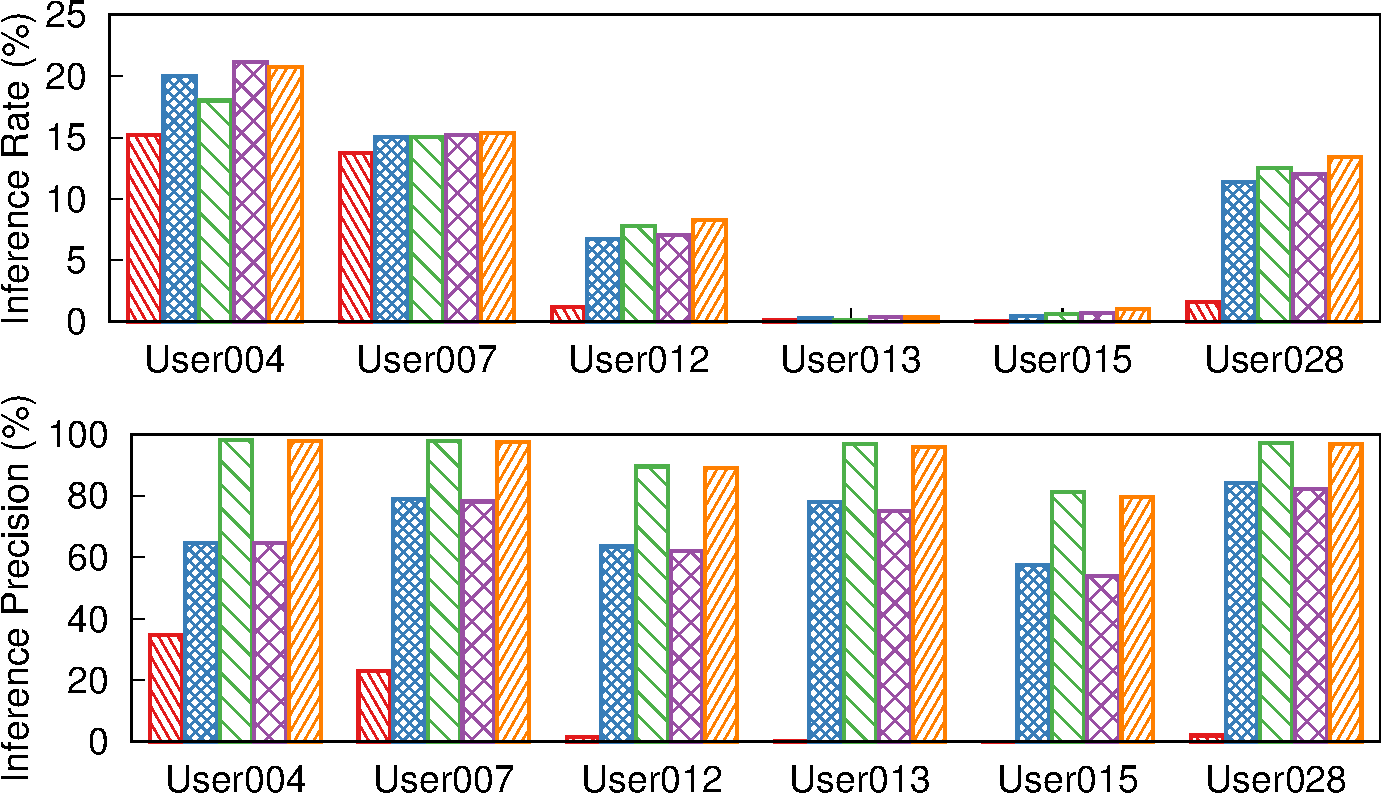
\includegraphics[height=2.1in]{pic/distribution-comparison-fsl.pdf} &
        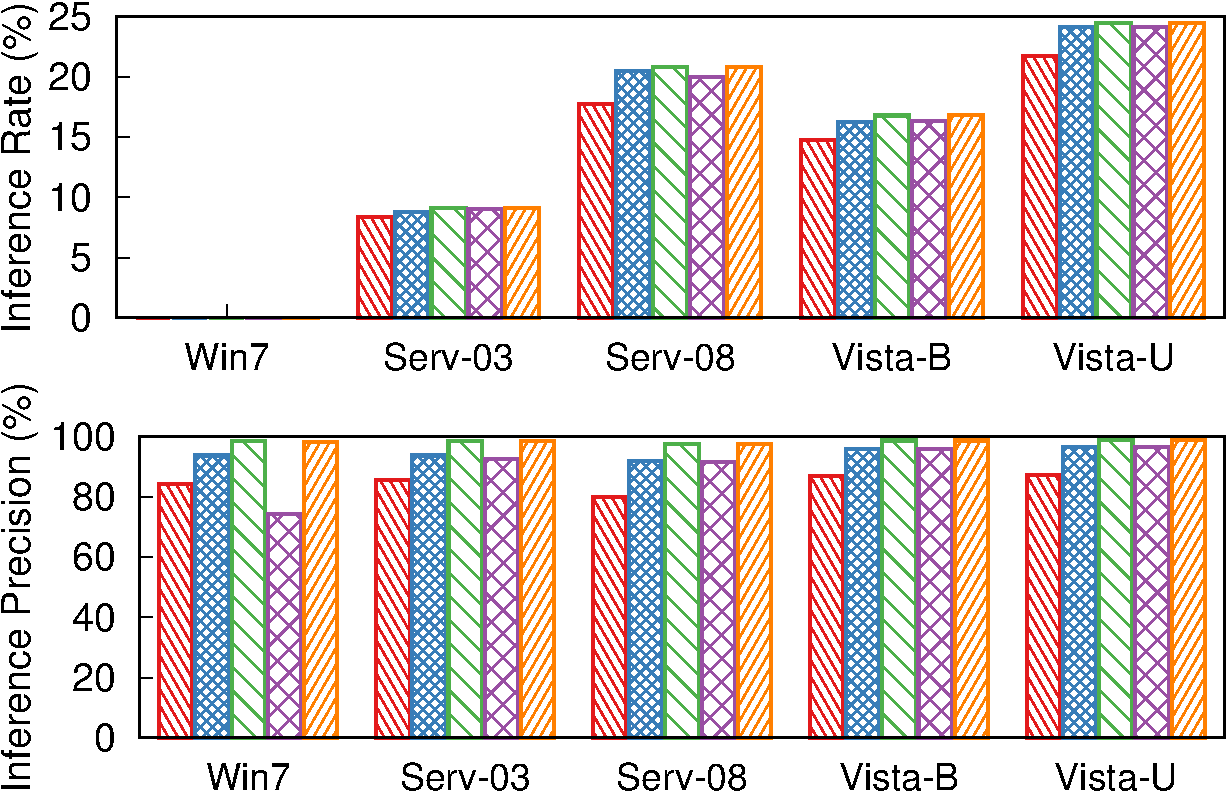
\includegraphics[height=2.1in]{pic/distribution-comparison-ms.pdf} \medskip \\
        {\footnotesize 
        (a) FSL dataset 
        } &
        {\footnotesize
        (b) MS dataset 
        } \\
    \end{tabular}
    \caption{Experiment 2 (Comparison with prior attack): comparison of attack severity for distribution-based attack and locality-based attack.}
    \label{fig:distribution-comparison}
\end{figure*}



% \begin{itemize}[leftmargin=*]
	% \item {\em Distribution-I:} We configure our proposed distribution-based attack with the {\em same} configuration of the baseline above. Informed by Experiment 3, we further choose the distribution-based ranking parameters in the following way: for the FSL dataset, we fix $r$ = 10 for all users, and individually set $t$ = 1.5, 1.2, 1, 1, 0.7, and 0.9 for User004, User007, User012, User013, User015, and User028; for the MS dataset, we fix $r$ = 10 for all categories, and configure $t$ as 2 for Win7 and Serv-08 and as 1.6 for Vista-U, Serv-03, and Vista-B, respectively.   

	% \item {\em Distribution-II:} We configure our proposed distribution-based attack with the same ranking configuration of distribution-I, while building on a larger $u$ to infer more chunk pairs. The rationale is to increase inference rate, while we expect the inference precision is degraded slightly as the attack can filter out unreasonable inferences. Specifically, for the FSL dataset, we set $u$ = 128 for User004, User013 and User015, and $u$ = 256 for User007, User012 and User028, respectively; for the MS dataset, we set $u$ = 128 for Win7, and $u$ = 30 for Serv-03, Serv-08, Vista-B, and Vista-U, respectively.
% \end{itemize}

Figure~\ref{fig:distribution-comparison}(a) shows the
comparison results of the FSL dataset. We observe that different instances of
the distribution-based attack outperform the locality-based attack in almost
all cases. For example, regarding User028, the lowest inference rate of the
distribution-based attack is 11.4\%, with the precision of 84.1\% (due to $\tt
Distribution$), while the corresponding inference rate and precision of
$\tt Baseline$ are only 1.2\% and 1.7\%, respectively; this implies that the distribution-based attack reduces the number of false postives by 82.4\% in this case.   

{\bf Observation (4) --} {\em The distribution-based attack significantly
increases the inference precision, while achieving a higher inference rate than
the locality-based attack.} 

$\tt Distribution^S$ and $\tt Distribution^S$-$\tt o$ have higher inference
precisions than $\tt Distribution$ and $\tt Distribution$-$\tt o$,
respectively, since they further filter false positives by size information.
For example, for User004, $\tt Distribution^S$ and $\tt Distribution^S$-$\tt o$  reduce the fraction of false positives in  $\tt Distribution$ and $\tt Distribution$-$\tt o$ from 35.2\% to 1.7\% and from 35.3\% to 2.2\%, respectively. However, in the same case,    
 we observe that the inference rates of $\tt Distribution$ and $\tt Distribution$-$\tt o$ are 20.0\% and 21.2\%, slightly higher than those of  
$\tt Distribution^S$ and
$\tt Distribution^S$-$\tt o$ by 2.0\% and
0.4\%, respectively. The reason is that $\tt Distribution$ and $\tt
Distribution$-$\tt o$ infer a small number of correct results from the
neighbors of incorrect ciphertext-plaintext pairs. In other words,  although
$(C, M)$ is an incorrect ciphertext-plaintext pair, the neighbors of $C$ may
correspond to those of $M$ with a small probability. Even in this case, all distribution-based attack instances are more severe than the locality-based attack instance. Specifically, the inference rate of $\tt Baseline$ is only 15.2\%, lower than those of the best and the worst distribution-based attack instances by 6.0\% and 2.8\%, respectively. 

% For the same reason, $\tt Baseline$ has higher inference rate than $\tt Distribution^S$ in User013.   

{\bf Observation (5) --} {\em Filtering incorrect inference results improves
the inference precision, yet it degrades the coverage of inferred
ciphertext-plaintext pairs and possibly decreases the inference rate.
} 

We further observe that although $\tt Distribution$-$\tt o$ and $\tt
Distribution^S$-$\tt o$ build on larger $u$, their inference rates are just
slightly higher than those of $\tt Distribution$ and $\tt Distribution^S$ by
0.4\% and 0.9\%, respectively. The reason is that the distribution-based
attack iterates inference just through neighbors, and has a bounded coverage
of inferred ciphertext-plaintext pairs. The further increase of $u$ only adds
a small number of new correct  ciphertext-plaintext pairs into results. 

Figure~\ref{fig:distribution-comparison}(b) shows the
results of the MS dataset. Both locality-based and distribution-based attacks
have high inference rates and precisions in most MS categories (except Win7).
The possible reason is that MS snapshots are highly correlated (e.g., the
variance of the total number of chunks is small, as shown in
Table~\ref{tab:dataset}).  We observe that the distribution-based attack still
outperforms the locality-based attack. For example, in Vista-U, the inference
rates and precisions of all inferences of the distribution-based attack are
above 24.1\% and 96.4\%, while those of $\tt Baseline$ are 21.7\% and 87.1\%,
respectively. 

Note that both  distribution-based and  locality-based attacks have low
inference rates (e.g., less than 0.01\%) in the Win7 category. The reason is
 that Win7 includes a large fraction (e.g., more than 98.8\%, as shown in
Table~\ref{tab:dataset}) of unique chunks, which cannot be correctly
inferred by the frequency analysis attacks. 

% We do not include Win7  in the comparison, since all attack instances have low effectiveness. We observe all attacks have higher severity than those in the FSL dataset.   



\begin{figure*}[t]
     \centering
    \centering
    \begin{tabular}{c@{\hskip 2em}c}
        \multicolumn{2}{c}{
\includegraphics[width=.25\textwidth]{pic/legend-effectiveness.pdf}} \smallskip \\
        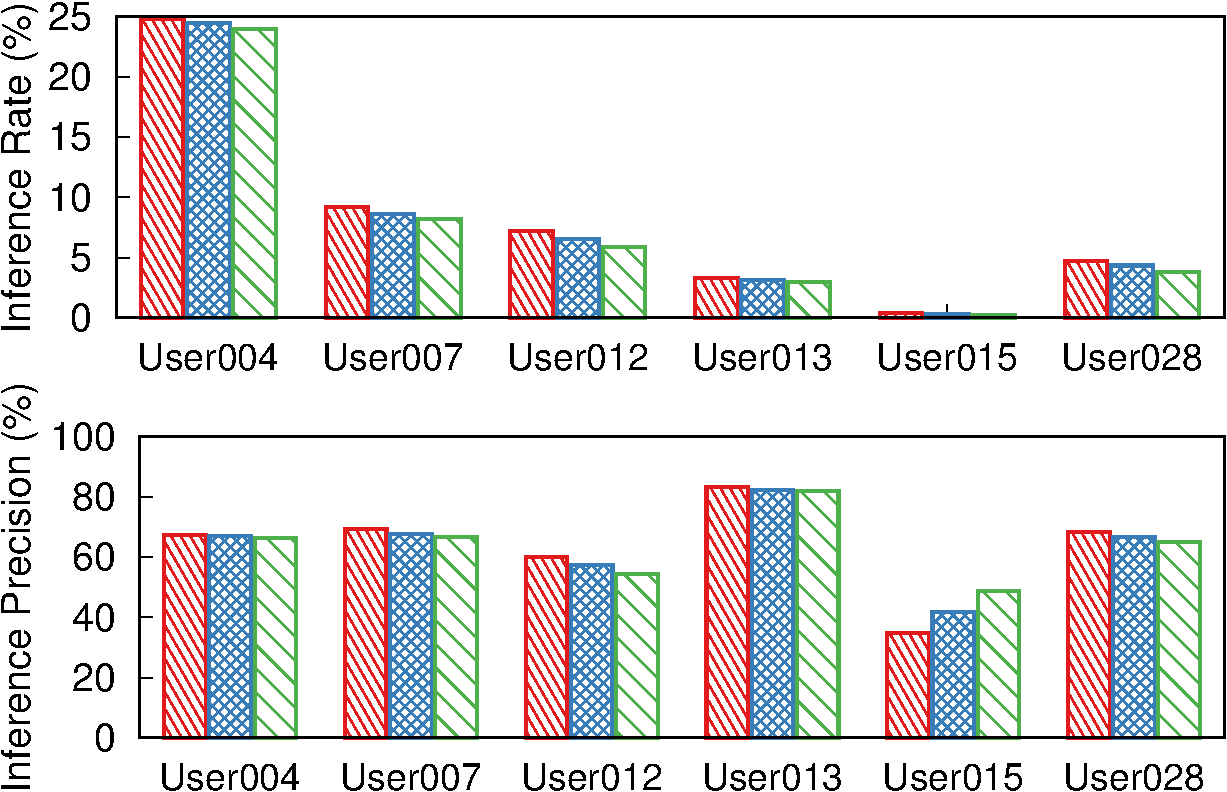
\includegraphics[height=2.2in]{pic/distribution-effectiveness-wo-size.pdf} &
	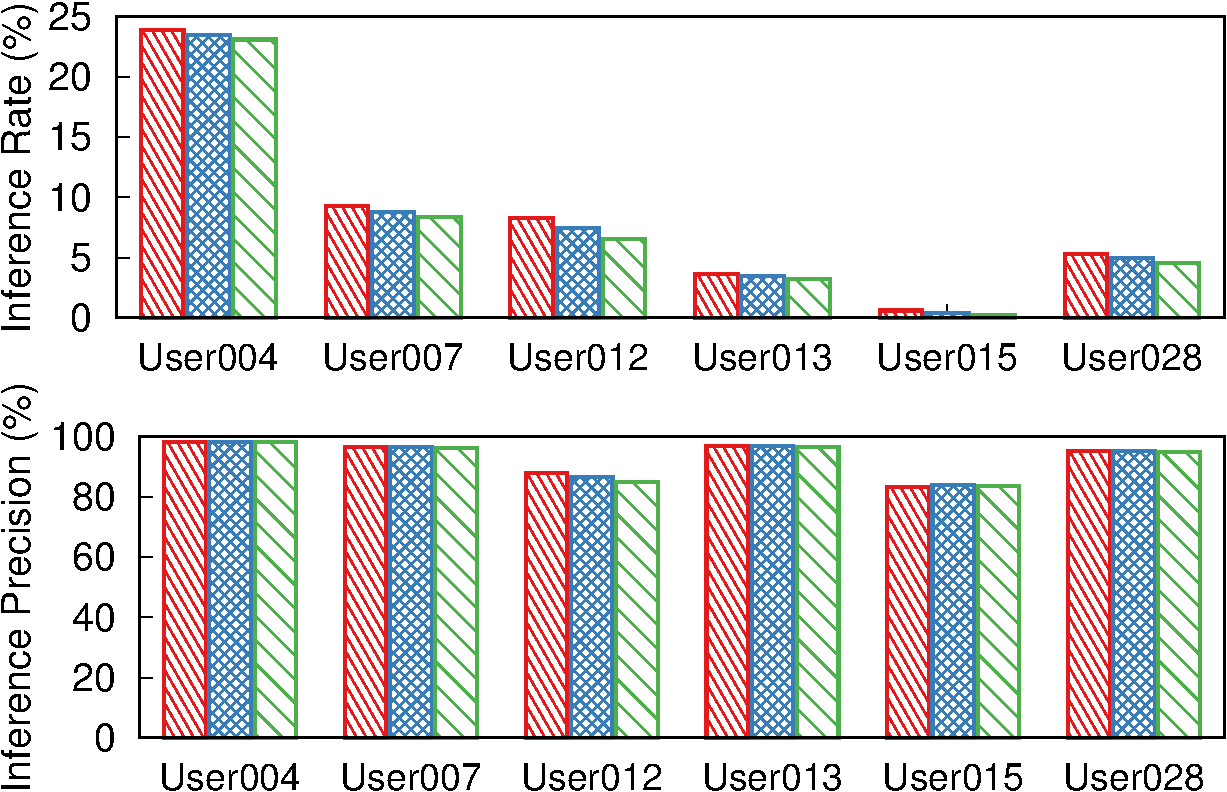
\includegraphics[height=2.2in]{pic/distribution-effectiveness-w-size.pdf} \medskip \\
        {\footnotesize 
        (a) Distribution-based attack without size information  
        } &
        {\footnotesize
        (b) Distribution-based attack with size information 
        } \\
    \end{tabular}
	\caption{Experiment 3 (Attack effectiveness): severity of distribution-based attack in FSL dataset.}
	\label{fig:experiment-distribution-effectiveness}
\end{figure*}


\subsection{Experiment 3 (Attack effectiveness):} We consider a long-term
backup scenario and examine the effectiveness of the distribution-based attack
with the FSL dataset. Specifically, we choose the $i$th FSL weekly backup of
each user as the auxiliary information to infer original plaintexts in the corresponding $(i+w)$th FSL
weekly backup. Clearly, the smaller $w$ is, the higher correlation between the
auxiliary information and the target backup will be.  We configure the two  
distribution-based attack instances $\tt Distribution$-$\tt o$ and $\tt Distribution^S$-$\tt o$
like Experiment~2, and evaluate their inference rates and inference precisions that
are averaged for all available $i$ for each user. 

Figure~\ref{fig:experiment-distribution-effectiveness}(a) shows the results. The
distribution-based attack has varying inference rate and precision  across
users. For example, in the favorable case like User004, it achieves the
highest inference rates of 24.8\%, 24.5\%, and 24.0\% with the precisions of
67.3\%, 67.0\%, and 66.5\% for $w$ = 1, 2, and 3, respectively; in the
non-favorable case like User015, the inference rate of the distribution-based
attack is only around 0.3\%. The possible reason is that the backup data from
User015 has low chunk locality. 

In addition, we observe that the correlation (i.e., $w$) of the auxiliary
information has low impact on the effectiveness of the distribution-based
attack.  For example, when $w$ increases from 1 to 3, it only leads to limited
degradations on inference rate (e.g., less than 1.4\%) and precision (e.g.,
less than 5.6\%). The reason is that the distribution-based attack addresses
disturbances to frequency ranking and preserves attack effectiveness.  

{\bf Observation (6) --} {\em The distribution-based attack can limit the
degradation of attack effectiveness in the presence of loosely correlated
auxiliary information.} 

% We also use the instance in Experiment 2 to evaluate the effectiveness of the distribution-based attack that operates with
 % size information. 
 Figure~\ref{fig:experiment-distribution-effectiveness}(b) shows the results of $\tt Distribution^S$-$\tt o$. We observe that it has similar inference rate with $\tt Distribution$-$\tt o$,  
 while achieving much higher precision. For example, the average inference precision of all users are 93.1\%, 92.8\%, and 92.4\% for $w$ = 1, 2, and 3, respectively.  

% Figure~\ref{fig:experiment-distribution-severity-ms} shows the attack results of the MS dataset. The distribution-based attack achieves high severity. For example, it can infer 24.0\% of unique chunks in Vista-U with a precision of 96.2\%.    

% Although there is l          

\section{Results of Clustering-based Attack}
\label{sec:experiment-clustering}




\subsection{Experiment 4 (Impact of parameter):} We first evaluate the impact
of the parameter $k$, which defines the upper bound distance
in combining the closest clusters.  We use both the FSL and the VM datasets to
study how $k$ affects the underlying clustering scheme in the attack.
Specifically, we apply segmentation on the last backup of each considered FSL
and VM user, respectively, and generate the segments that have a fixed size of
4MB. 

The clustering scheme aims to aggregate similar ciphertext segments into the
same cluster, without compromising the confidentiality of chunks in each
ciphertext segment.  To quantify its effect, we compare the results of
clustering with those of a {\em real} classification approach, which directly
classifies segments by their minimum chunk hash.  Suppose we generate $m$ real
classes of segments by classification, and $\widetilde{m}$ clusters by the
clustering scheme, respectively.  We consider {\em clustering closeness},
evaluated by $\frac{{\sf abs}(m-\widetilde{m})}{m}$ (where 
${\sf abs}(m-\widetilde{m})$ returns the absolute value of $m-\widetilde{m}$),
which quantifies how the  number of clusters approximates that of real
classes. In addition, let $\hat{m}$ be the number of clusters, in which all
segments are similar (i.e., have the same minimum chunk hash). We also
consider {\em clustering correctness}, evaluated by
$\frac{\hat{m}}{\widetilde{m}}$, which quantifies how precisely the clustering
scheme groups similar segments.  

Figure~7(a) shows the results of the FSL dataset, where we
consider four FSL users (e.g., User004, User007, User015 and User028) for
saving evaluation time. The clustering closeness first increases with $k$,
since the number (i.e., $\widetilde{m}$) of clusters decreases and
approximates $m$. When $k$ increases further, the number of clusters drops
away from $m$, and leads to the increase of clustering closeness.  In
addition, we observe that the clustering correctness gradually decreases with
$k$, because some of non-similar segments (i.e., their minimum chunk hashes are
different) are aggregated into the same cluster. Both results suggest that we
can configure an appropriate $k$ to balance the closeness and correctness of
clustering. For example, when we set $k$ = 0.65 for User015, the corresponding
closeness and correctness are 1.0\% and 94.2\%, respectively. This implies
that the results of the clustering scheme  highly approximates
those of real classification.             

{\bf Observation (7) --} {\em By configuring an appropriate $k$ for
clustering, we  approximate the results of  classifying segments, without the knowledge of  minimum chunk hash in each
segment.}   

Figure~7(b) shows the results of the VM dataset. We observe
that the clustering closeness and correctness of all VM users have  similar
tendencies with those of FSL users. When we configure $k$ = 0.8, the average
clustering closeness of all VM users is only 3.0\%, while the corresponding
clustering correctness is as high as 93.1\%.     


\begin{figure*}[t]
\centering
    \begin{tabular}{cc@{\hspace{0.3in}}p{.32\textwidth}}
    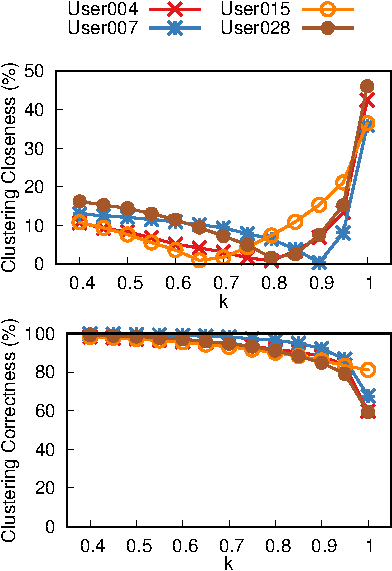
\includegraphics[width=.3\textwidth]{pic/clustering-impact-d-fsl.pdf} &
    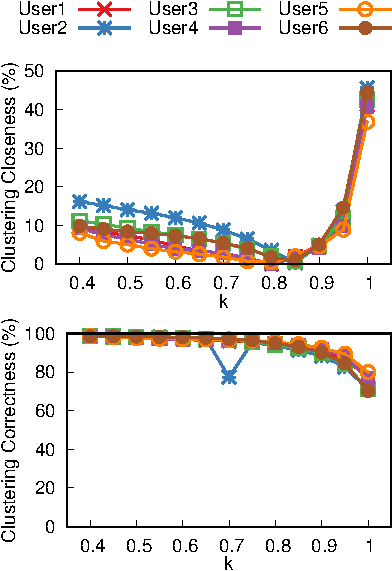
\includegraphics[width=.3\textwidth]{pic/clustering-impact-d-vm.pdf} & 
    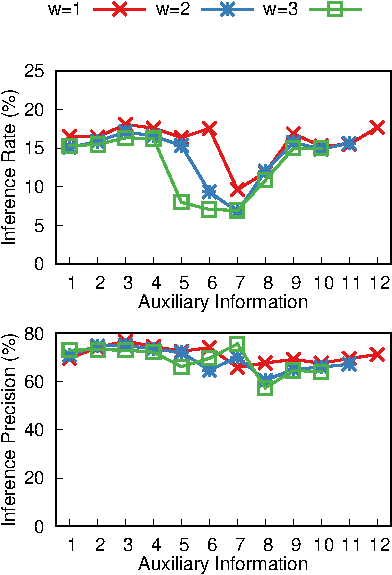
\includegraphics[width=.3\textwidth]{pic/clustering-effectiveness.pdf} \medskip \\
{\footnotesize 
        (a) FSL dataset } 
&
{\footnotesize 
        (a) VM dataset } 
        &  ~~~ \medskip \\
        \multicolumn{2}{p{.64\textwidth}}{
            \footnotesize Fig.~7\quad Experiment 4 (Impact of parameter): impact of $k$ in the clustering scheme; for clustering closeness, the smaller the better; for clustering correctness, the larger the better. } &
        % \multicolumn{2}{c}{\footnotesize Fig.~6\quad Experiment 4 (Impact of parameter): show impact of $d$ with clustering closeness and correctness; for clustering closeness, the smaller the better; for clustering correctness, the larger the better.} &
        {\footnotesize
Fig.~8\quad Experiment 5 (Attack effectiveness):  severity of clustering-based attack in VM dataset.
        }
\end{tabular}
    \hspace{-1in}
\end{figure*}

% \begin{figure}
% 	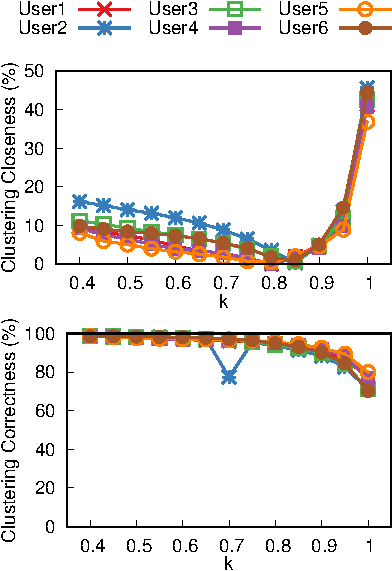
\includegraphics[width=.48\textwidth]{pic/clustering-impact-d.pdf}
% 	\caption{Experiment 6 (Impact of parameter).}
% 	\label{fig:experiment-clustering-impact}
% \end{figure}

\begin{table*}[!t]
\small
    \caption{Experiment 6 (Security implications)}
\renewcommand{\arraystretch}{1.2}
\vspace{-3pt}
 \begin{minipage}[t]{0.7\textwidth}
\centering
        (a) Distribution-based attacks \medskip \\
\begin{tabular}{|c|c|c|c|c|c|}
\hline

    \multirow{2}{*}{\bf Type} & \multirow{2}{*}{\bf Extension Name} & \multirow{2}{*}{\bf \centering Range of File Size}  & \multicolumn{2}{c|}{\bf Raw Inference Rate} \\ \cline{4-5} 
    & & &  $\sf Distribution$-$\sf o$ & $\sf Distribution^S$-$\sf o$ \\ \hline
\hline
    Office & doc(x), ppt(x), xls(x) & 10KB-1MB   & 4.9\% & 5.3\%\\
\hline
    Picture & jpg, png &10-100KB  & 7.7\% & 6.7\% \\
\hline
    Source & c, h, cpp, java, py & 10-20KB   & 17.1\% & 15.0\%\\
% \hline
	% Library & .a, .dll, .so \\
% \hline
	% Compression & .bz2, .gz, tar, rar, zip, 7z \\
\hline
    Database & db, po & 20-700KB   & 2.6\% & 2.4\%\\
\hline
    Disk & vmdk, img & 200MB-1GB  & 15.8\% & 16.7\%\\
\hline
\end{tabular}
\label{tab:file}
 \end{minipage}
\hfill
    \begin{minipage}[t]{0.3\textwidth}
    \centering
        (b) Clustering-based attack \medskip \\
    \begin{tabular}{|c|c|}
    \hline
        {\bf Users} & {\bf Raw Inference Rate} \\
    \hline
    \hline
        1 & 13.2\% \\ 
    \hline
        2 & 22.4\% \\ 
    \hline
        3 & 25.7\% \\ 
    \hline
        4 & 28.4\% \\ 
    \hline
        5 & 18.5\% \\ 
    \hline
        6 & 30.8\% \\ 
    \hline
    \end{tabular}
\label{tab:user}
    \end{minipage}

\end{table*}



\subsection{Experiment 5 (Attack effectiveness):} We now study the
effectiveness of the clustering-based attack. Due to the boundary shift of
fixed-size segment, it has low effectiveness
(about 1\% inference rate in our test) against the FSL dataset.  Thus, we use
the VM dataset to examine its severity. To configure the attack, we set $k$ =
0.8 for clustering, and $(u, r, t)$ = (5000, 100, 0.5) for relating ciphertext
clusters to corresponding plaintext clusters.  

In our micro-benchmarking, we find that the chunk-level inference in the
clustering-based attack only infers thousands of chunks correctly, which
contributes to a negligible inference rate (e.g., less than 0.01\%).  
% The
% reason is that each cluster includes a large number of chunks, and frequency
% analysis is ineffective in this case. 
Thus, we focus on the
segment-level inference, which presents the bottom line of severity in the
clustering-based attack. To be consistent with the chunk-level measurements, we count inference rate and precision based
on the unique chunks in each correctly inferred segment. 

We use the same evaluation methodology of Experiment~3, and report the results
in Figure~8. Specifically, the x-axis describes the index $i$ (where 1 $\leq i \leq$
12) of the VM backup that is used as the auxiliary information for attack,
while the y-axis presents the average inference rate or precision of all VM
users against the $(i+w)$th backup (where $w$ = 1, 2, and 3). We observe that both the inference rate and the inference
precision fluctuate significantly. For example, when using the 3rd backup as
the auxiliary information, the attack achieves the highest inference rates at
18.1\%, 17.1\% and 16.3\%, with the precisions of 76.8\%, 75.0\% and 73.0\%
for $w$ = 1, 2, and 3, respectively. 
On the other hand, when using the 7th
backup as the auxiliary information, the corresponding inference rates and
precisions drop down to 9.6\% and 65.9\%, 6.8\% and 71.2\%, and 6.9\% and
75.6\%, respectively. The reason is that the VM users have heavy updates after
the 7th week, and this reduces the correlation  of adjacent backups. 
On
average, for $w$ = 1, 2 and 3, the clustering-based attack infers 15.8\%,
14.0\%, and 12.6\% ciphertext-plaintext pairs, with the precisions of 71.1\%,
69.1\%, and 68.9\%, respectively. 
% This demonstrates high severity against
% the VM disk images.   

\section{Results of Security Implications}
\label{sec:case}
We thus far have examined the severity of inference attacks by quantifying the
correctly inferred ciphertext-plaintext pairs.  However, it remains an open
issue that what are the security implications informed by these results and
how the frequency analysis attacks bring actual damage. In the following
experiment, we evaluate the security implications of our attacks based on the
{\em raw inference rate}, defined as the percentage of raw data content
affected by correctly inferred chunks.   




\subsection{Experiment 6 (Security implications):}
We first consider the distribution-based attack, and evaluate its raw
inference rate against {\em different types} of files. We drive the evaluation
using the FSL dataset, since only the FSL dataset includes file metadata (that
includes the extension names of files) in plaintext. Specifically, we focus on
five types of files that have specific extension names (see
Table~\ref{tab:file}(a)): office files ({\em Office}), picture files 
({\em Picture}), programming source files ({\em Source}), database files 
({\em Database}), and disk image files ({\em Disk}). These files occupy more
than 60\% of raw content of FSL snapshots.   

We apply the methodology of Experiment~2, and evaluate the raw inference
rates of $\sf Distribution^S$-$\sf o$ and $\sf Distribution$-$\sf o$. 
Table~\ref{tab:file}(a) shows the results. Both attack instances have high raw
inference rates against {\em Disk} (e.g., 15.8\% for 
$\sf Distribution$-$\sf o$ and 16.7\% for $\sf Distribution^S$-$\sf o$),
because each disk file includes a large number of rarely updated chunks that
form high locality within the same file. Interestingly, we observe that 
{\em Source}, although each file is of a small size, also incurs high raw
inference rates by the distribution-based attacks (e.g., 17.1\% for 
$\sf Distribution$-$\sf o$ and 15.0\% for $\sf Distribution^S$-$\sf o$). The
reason is that programming source files are often stored together in file system
(e.g., the source files that belong to the same project locate in an identical
directory) and form a large stretch of correlated chunks, which present high
locality across files. For small and scattered files (e.g., {\em Office}, 
{\em Picture}, and {\em Database}), the distribution-based attacks have
relative low raw inference rates.     


{\bf Observation (8) --} {\em The severity of the distribution-based attack depends on the update frequencies, sizes, and spatiality of target files. } 

We examine the security implication of the clustering-based attack using the
VM dataset. Specifically, we use the 11th  backup of each VM user  to infer original content in corresponding 13th VM
backup. Since the VM dataset does not contain any metadata, we count the raw
inference rate based on the  whole data content in each VM snapshot.
Note that we filter all zero chunks in the count of raw inference rate,
because they occupy a large fraction in VM disk images \cite{jin09}.           


% switch to the clustering-based attack, and infer the content of the last (i.e., the 13th) VM backup based on the corresponding 11th backup. Since the VM dataset does not contain metadata, we evaluate the raw inference rate across different users. Specifically, like Experiment 7, we only consider segment-level attack for high precision, and count the raw inference rate based on the correctly inferred segments. Note that since VM images commonly contain a large fraction of zero chunks ,  we filter out the zero segments in our inferred raw content.    

We use the same configuration of Experiment~5, and evaluate raw inference rate
based on segment-level inference.  Table~\ref{tab:user}(b) shows the results
for different users.  We observe that the clustering-based attack achieves high
severity against the VM dataset. For example, it infers up to 30.8\% raw
content of User6's VM backup. On average, the raw inference rate of all users
is as high as 23.2\%.  
% a relatively high raw inference rate.  On average, the raw inference rate is 23.2\% for all users. 

{\bf Observation (9) --} {\em The clustering-based attack threatens the
confidentiality of VM disk images. } 


\chapter{应对频率分析攻击的对策讨论}
\label{sec:Countermeasure}

在本章中,将讨论应对本文攻击方案使用的三种泄漏的对策及其优缺点。但在三中泄漏中,单纯的防范数据块大小信息泄漏并不足以使本文提出的攻击手段失效(大小信息的利用只是攻击用于进一步提高推理攻击准确性的可选条件)。

\section{防止频率泄漏}

MinHash加密\citing{qin2017design,li2017information}使用从一组相邻数据块上的最小块哈希导出的密钥加密该组内每个明文数据块,因此可能将相同的明文数据块加密映射到不同的密文数据块。防御频率信息泄漏的基本原理是通过MinHash加密改变各个密文数据块的频率,并由此扰乱不同数据块的频率排名。

与此同时,MinHash加密还可以用于防止本文中的频率分析攻击。MinHash加密是非确定性的加密方法,使用该方法会改变数据块的频率分布,因此本文的的攻击目标是确定性加密(例如,MLE\citing{bellare2013message})。但MinHash加密因为打破了明文数据块-密文数据块之间的一一映射关系,所以在加密重复数据删除中导致了存储效率的下降(重复数据删除所能节省的存储空间变小)。此外,因为MinHash加密的随机性主要取决于目标工作负载中的最小块哈希,所以其不是一种扰乱数据块频率的主动对策,在不同的工作负载中能实现的扰乱效果具有较大的差异。         

最近的一项工作\citing{zuo2018mitigating}提出通过有计划的添加冗余(重复)的数据块来防止针对客户端加密重复数据删除的流量分析攻击。该方法\citing{zuo2018mitigating}在运作中会改变数据块的频率,因此可以用于防止频率分析攻击。与MinHash加密相比,该方法\citing{zuo2018mitigating}只是添加了重复的数据块,因此不会降低存储效率。但另一方面,它需要使用在特定的假设之下。首先它要求特定的数据块是重复的,其次它只适用于客户端重复数据删除。因此使用这种方法可能会引入额外的泄漏通道(参见\ref{sec:RelatedWork})。

现有工作提出了几个扩展的MLE实例基于强加密原语构建,以防止加密重复数据删除的频率泄漏,例如支持等式测试的随机加密\citing{abadi2013message},混合加密\citing{stanek2014secure},以及与完全同态加密的交互\citing{bellare2015interactive}。它们都提供了可证明的安全性,但它们如何在实践中实施和部署仍未有进一步的研究。

\section{防止顺序泄漏} 

一个简单的对策是干扰数据块在重复数据删除处理中顺序。例如,加密重复数据删除可以在加密之前对明文数据块流进行额外的顺序扰动添加处理,以隐藏每个明文数据块的真实逻辑顺序。这种方法可以有效的防止基于分布的频率分析攻击(参见\ref{sec:DistributionAttack}),因为攻击者无法正确识别到数据块邻居信息。但它对于基于聚类的频率分析攻击(参见\ref{sec:ClusteringAttack})并不是完全有效的。如果添加扰动仅在很小的范围内进行(例如,每个数据段中的明文数据块的顺序被添加扰动),则基于聚类的频率分析攻击方法仍然有效。

顺序扰乱策略的最大缺陷在于它破坏了数据块的局部性并且在大规模的重复数据删除中会导致性能的严重下降\citing{xia2011silo,zhu2008avoiding,lillibridge2009sparse}。

\section{防止大小泄漏}

正如已有的工作\citing{ritzdorf2016information}所建议的那样,加密重复数据删除可以在每个明文数据块种填充额外的数据来混淆这个明文数据块的实际大小。但是,这种填充方案的实现存在很大的难度,因为它需要在相同的明文数据块中添加相同的冗余数据;否则加密重复数据删除存储系统无法正常检测数据块是否重复。一种可能的解决方案建立在MLE\citing{keelveedhi2013dupless,bellare2013message}的范例之上,考虑将每个明文数据块的加密哈希作为计算种子,并使用它来生成可变大小的伪随机数据用于明文数据块的填充。与MLE一样,这种解决方案的代价是需要使用服务器辅助方法\citing{keelveedhi2013dupless}来抵御暴力攻击(参见\ref{sec:RelatedWork})。   


另一种思路是使用固定大小的数据块分块方法来取代可变大小的数据块分块方法。在这种情况下,由于所有的数据块都具有相同的大小,因此攻击者无法利用大小信息来区分它们。虽然固定大小的分块会受到边界偏移的影响,但它在VM磁盘映像这一特定数据类型中实现了与可变大小数据块分块方案几乎相同的重复数据删除存储空间节省效果\citing{jin2009effectiveness}。 因此,本文建议在某些特定的加密重复数据删除工作负载(例如,VM磁盘映像)中应用固定大小的数据块分块方法,以防止数据块大小信息泄漏。

\chapter{相关工作}
\label{sec:RelatedWork}

\section{MLE的应用}

回顾\ref{sec:background},MLE\citing{bellare2013message}正式确立了加密重复数据删除的加密方案基础。第一个发布的MLE实例是收敛加密(CE)\citing{douceur2002reclaiming},它使用明文的加密哈希及其对应的密文作为MLE密钥和标签。其他CE的变体包括:散列收敛加密(HCE)\citing{bellare2013message},它从明文中导出标记,同时仍然使用明文的哈希作为MLE密钥;随机收敛加密(RCE)\citing{bellare2013message},用新的随机密钥加密明文以形成非确定性密文,通过从明文的哈希中导出的MLE密钥保护随机密钥,并附加来自明文的确定性标签以实现数据块重复性的检查;收敛扩散加密(CD)\citing{li2015cdstore},它通过使用明文的加密哈希作为秘密共享算法的随机种子,将CE扩展到秘密共享。由于所有上述实例仅从明文中获取MLE密钥和(或)标签,如果明文是可预测的(即,所有可能的明文的总数量有限),它们很容易受到离线暴力攻击\citing{keelveedhi2013dupless}的影响,因为攻击者可以从所有可能的明文中穷举地导出MLE密钥和标签,并检查是否存在某种明文被加密到目标密文(在CE,HCE和CD中)或映射到目标标签(在RCE中)。

暴力攻击已经被证明可以用来获取文件信息\citing{wilcox2008drew}。为了防止离线暴力攻击,DupLESS\citing{keelveedhi2013dupless}通过在独立密钥服务器中管理MLE密钥来实现服务器辅助MLE,从而确保无法从离线消息中获得每个MLE密钥。DupLESS采用两种机制来实现强大的MLE密钥管理:
\begin{enumerate}
    \item \textbf{无关密钥生成:}
        
        DupLESS中客户端总是在不向密钥服务器显示消息内容的前提下从密钥服务器获得确定性MLE密钥。
    \item \textbf{密钥生成频率限制:}
        
        DupLESS中的密钥服务器通过限制来自客户端的密钥生成请求频率,防止在线暴力攻击。
\end{enumerate}

其他研究扩展了服务器辅助MLE的各个方面,例如可靠的密钥管理\citing{duan2014distributed},透明定价\citing{armknecht2015transparent},点对点密钥管理\citing{liu2015secure}和密钥转换(所属权变更) \citing{qin2017design}。但是服务器辅助MLE仍然建立在确定性加密的基础之上,现有的MLE实例(基于CE或服务器辅助MLE)都容易受到本文研究的推理攻击方法的攻击。

\section{对(加密)重复数据删除的攻击} 

除了离线暴力攻击之外,之前的研究还考虑了针对重复数据删除存储的各种攻击,此类攻击通常也适用于加密重复数据删除。例如,侧信道攻击\citing{harnik2010side,halevi2011proofs}使攻击者可以利用重复数据删除的运作模式来推断目标用户上传文件的具体内容,或者在客户端重复数据删除中获取未经授权的访问权限;例如,2010年针对“Dropbox”成功发起了侧通道攻击(以及其他相关攻击)\citing{mulazzani2011dark}。重复伪造攻击\citing{bellare2013message}通过利用不一致的标签破坏了消息的完整性。Ritzdorf等人在其工作中利用数据块大小的泄漏来推断文件的存在性\citing{ritzdorf2016information}。基于数据块局部性的攻击\citing{li2017information}利用频率分析来推断密文数据块-明文数据块对。本文的工作在推理攻击的已有工作\citing{ritzdorf2016information,li2017information},通过利用各种类型的泄漏给出了针对加密重复数据删除的推理攻击的更深入研究。
   
\section{防御机制} 

 在\ref{sec:Countermeasure}中讨论了针对加密重复数据删除的频率,顺序和大小泄漏的应对对策。而其他防御机制旨在防范其他类型的攻击。
 
如上所述,服务器辅助的MLE\citing{keelveedhi2013dupless}可以抵御离线暴力攻击。服务器端重复数据删除\citing{li2015cdstore,harnik2010side,armknecht2017side}和所有权证明\citing{xu2013weak,di2012boosting,halevi2011proofs}可以抵御侧信道攻击。服务器端标签生成\citing{douceur2002reclaiming,keelveedhi2013dupless}和受保护的解密\citing{bellare2013message}可以抵御重复检查攻击。


\section{推理攻击}  

已有工作已经提出了几种针对加密数据库\citing{grubbs2017leakage,bindschaedler2018tao,kellaris2016generic,durak2016else,naveed2015inference,lacharite2018improved}和关键字搜索\citing{zhang2016all,grubbs2016breaking,pouliot2016shadow,cash2015leakage,islam2012access}的推理攻击方案。它们都利用确定性加密的性质来识别不同类型的泄漏。本文的研究内容与它们的不同之处在于专门研究了针对加密重复数据删除的频率分析推理攻击。

\chapter{结论}
\label{sec:Conclusion}

Encrypted deduplication applies deterministic encryption, and leaks the frequencies of plaintexts. This paper revisits the security vulnerability  due to frequency analysis, and demonstrates that encrypted deduplication is even more vulnerable towards inference attacks. We propose two new frequency analysis attacks, both of which  achieve high inference rate and high inference precision, while under different assumptions of adversarial knowledge. We empirically evaluate our attacks with three real-world datasets, present a variety of new observations about their natures, and further analyze how they bring actual damages. We also discuss the advantages and disadvantages of possible countermeasures to advise practitioners for securely implementing and deploying encrypted deduplication storage systems. 


% types of files are especially insecure under these attacks.    
% We propose two new inference attacks, which augment the prior attack \cite{li17} with high precision inference and relaxed adversarial knowledge, respectively.   
% While prior work \cite{li17} has illustrated the vulnerability  via frequency analysis, this paper presents an in-depth study on the security of encrypted deduplication, and       
 We pose three directions for future work. First, we consider a complete old backup as the auxiliary information, and do not study how to launch attack if the adversary only has partial knowledge about the old backup. Possibly, we can still apply the frequency analysis attacks to extract characteristics from the available partial backup, and infer ciphertext-plaintext pairs by comparing the characteristics with those in the target backup. One direction is can we design advanced inference attacks, which  perform better than directly applying our attacks in this partial knowledge case?  
 
 
 % The attack effectiveness depends on how the information in the partial backup correlates with the target backup.       
 Second, we adjust the parameters of the frequency analysis attacks based on their effectiveness, which can only be learnt after the attacks have happened. We do not study how to derive the optimal parameters from auxiliary information beforehand. Future work may do better. 
 
 % We believe the parameter configurations depend on the characteristics of workloads, but do not see how to derive them efficiently.     
 
 % the frequency analysis attacks are parameter sensitive. We adjust parameters based on the attack effectiveness (that can only be measured after the attack happens), and do not study how to identify the optimal parameter configuration  beforehand. We believe the parameter configurations depend on the characteristics of workloads, but do not see how to derive them efficiently. Future work may do better.    
 
 % our proposed attacks are parameter sensitive. In evaluation, we adjust the parameters based on attack results, and report the security vulnerability of encrypted deduplication under some {\em specific} parameter settings of our attacks. We do not  study how to identify the optimal parameter setting of attack without the knowledge of attack results. We begin to consider that the attack configurations possibly depend on the characteristics of target workloads, but do not see how to derive them. Future work may do better. 

% help practitioners and researchers better understand the security issues in encrypted deduplication storage and motivate more research along this direction.
% While 
% of encrypted deduplication
% Although it is vulnerable to frequency analysis, prior work \cite{li17} shows that classical frequency analysis can only infer a few original chunks in practice. This paper considers to increase the effectiveness of frequency analysis with additional leakages. Specifically, we present three new inference attacks by exploiting the size and order leakages that have been witnessed in deduplication systems \cite{xia11,lillibridge09,zhu08,douceur02, wilcox-ohearn08, bellare13b}. We evaluate the effectiveness of  our attacks with real-world datasets, and show that they can infer significant amount of original data under different types of workloads. We also discuss possible countermeasures to address the leakage channels exploited by our attacks. We pose the following future works.   

Third, we do not implement  attack prototypes against real-world encrypted deduplication storage systems. Another direction is to deploy our attack design and 
report the vulnerability of encrypted deduplication in practice.








% - Our attacks are parameter sensitive. One direction is to explore the relationship between configuration and workload characteristics.

% - There seems a tradeoff between size-based attack and distribution-based attack. Throughout our experiment, size-based attack operates big chunks better, since they have more variances on chunk size. The distribution-based attack is expected to operate small chunks better, because there exists more chunk locality between small chunks.

% - To defend our attacks, one approach is to obfuscate the chunk distributions. A recent work suggests to add redundant chunks to mix up network traffic. It works for changing chunk distribution, but depends on knowing if a chunk is duplicate before deduplication. 

% - This paper aims to report the vulnerabilities of encrypted deduplication, while not target on implementing a real attack against practical encrypted deduplication systems. Another direction is deploy our attack design in practice to alert the vulerabilities of encrypted deduplication.  







%\thesisacknowledgement

\nocite{*}
\bibliographystyle{thesis-uestc}
\bibliography{reference}

\thesisappendix

%\thesisloadachievement{publications}


%\thesistranslationoriginal
%\section{}
%
%
%\thesistranslationchinese
%
%\section{}

\end{document}
